%%% The main file. It contains definitions of basic parameters and includes all other parts.

%% Settings for single-side (simplex) printing
% Margins: left 40mm, right 25mm, top and bottom 25mm
% (but beware, LaTeX adds 1in implicitly)
\documentclass[12pt,a4paper]{report}
\setlength\textwidth{145mm}
\setlength\textheight{247mm}
\setlength\oddsidemargin{15mm}
\setlength\evensidemargin{15mm}
\setlength\topmargin{0mm}
\setlength\headsep{0mm}
\setlength\headheight{0mm}
% \openright makes the following text appear on a right-hand page
\let\openright=\clearpage

%% Settings for two-sided (duplex) printing
% \documentclass[12pt,a4paper,twoside,openright]{report}
% \setlength\textwidth{145mm}
% \setlength\textheight{247mm}
% \setlength\oddsidemargin{14.2mm}
% \setlength\evensidemargin{0mm}
% \setlength\topmargin{0mm}
% \setlength\headsep{0mm}
% \setlength\headheight{0mm}
% \let\openright=\cleardoublepage

%% Generate PDF/A-2u
\usepackage[a-2u]{pdfx}

%% Character encoding: usually latin2, cp1250 or utf8:
\usepackage[utf8]{inputenc}
\usepackage[T1]{fontenc}
%% Prefer Latin Modern fonts
\usepackage{lmodern}

%% Further useful packages (included in most LaTeX distributions)
\usepackage{amsmath}        % extensions for typesetting of math
\usepackage{amsfonts}       % math fonts
\usepackage{amsthm}         % theorems, definitions, etc.
\usepackage{bbding}         % various symbols (squares, asterisks, scissors, ...)
\usepackage{bm}             % boldface symbols (\bm)
\usepackage{graphicx}       % embedding of pictures
\usepackage{fancyvrb}       % improved verbatim environment
%%\usepackage{natbib}         % citation style AUTHOR (YEAR), or AUTHOR [NUMBER]
\usepackage[nottoc]{tocbibind} % makes sure that bibliography and the lists
			    % of figures/tables are included in the table
			    % of contents
\usepackage{dcolumn}        % improved alignment of table columns
\usepackage{booktabs}       % improved horizontal lines in tables
\usepackage{paralist}       % improved enumerate and itemize
\usepackage{xcolor}         % typesetting in color
\usepackage{verbatim}
\usepackage{mathtools}
\usepackage{environ}
\usepackage{tabularx}
\usepackage{caption}
\usepackage{cleveref}
%%tikz packages
\usepackage{tikz}
\usetikzlibrary{shapes,snakes}
\usetikzlibrary{backgrounds}
\usetikzlibrary{calc}
\usepackage[numbers]{natbib}
% Todo notes. I can remove that before submitting.
\usepackage{todonotes}
%%% Basic information on the thesis

% Thesis title in English (exactly as in the formal assignment)
\def\ThesisTitle{Price of connectivity of graph parameters}

% Author of the thesis
\def\ThesisAuthor{Tereza Hulcová}

% Year when the thesis is submitted
\def\YearSubmitted{2020}

% Name of the department or institute, where the work was officially assigned
% (according to the Organizational Structure of MFF UK in English,
% or a full name of a department outside MFF)
\def\Department{Department of Applied Mathematics}

% Is it a department (katedra), or an institute (ústav)?
\def\DeptType{Department}

% Thesis supervisor: name, surname and titles
\def\Supervisor{Mgr. Tereza Klimošová, Ph.D.}

% Supervisor's department (again according to Organizational structure of MFF)
\def\SupervisorsDepartment{Department of Applied Mathematics}

% Study programme and specialization
\def\StudyProgramme{Computer Science}
\def\StudyBranch{Theoretical Computer Science}

% An optional dedication: you can thank whomever you wish (your supervisor,
% consultant, a person who lent the software, etc.)
\def\Dedication{%
	First of all I would like to thank my advisor Tereza Klimošová for the time
	and patient guidance that I received while working on this thesis.
	
	Next I wish to thank my grandmother Vlasta, my mother Vlasta, my uncle Jiří and my sister Barbora 
	and rest of the family for supporting me. I am also very grateful to my partner's family for their
        encouragement and for hosting me in Prague during my studies.
	
	Most of all, I thank my partner Martin Böhm for all his support, for motivating me and also for
        proofreading parts of the thesis.
}

% Abstract (recommended length around 80-200 words; this is not a copy of your thesis assignment!)
\def\Abstract{%
A vertex cover of a given graph is a vertex set including at least one
endpoint from every edge.  A vertex cover number \(\tau\) is the size
of a minimum vertex cover. If the vertices from a vertex cover are
required to induce a connected subgraph, the resulting set is called a
connected vertex cover.  The corresponding parameter \(\tau_c\) is
called a connected vertex cover number. The decision versions of both
problems are NP-complete.

To better understand a relation between these two vertex cover
numbers, Cardinal and Levy define the price of connectivity as a ratio
between \(\tau_c\) and \(\tau\). It is not surprising that determining
whether the price of connectivity of a given graph is at most \(t\) is
NP-hard. The notion of price of connectivity can be extended for more
graph properties, such as for the dominating set. The price of
connectivity has already been investigated in several papers, with
some focusing on critical graphs whose price of connectivity is
strictly greater than the price of connectivity of every induced
subgraph.

This thesis provides an overview of the current state of research into
the price of connectivity. Moreover, we focus on the structural
properties of critical graphs for the price of connectivity for vertex
cover and discuss a possible characterization of graphs in which the
price of connectivity for a dominating set is at most \(\frac{7}{3}\)
for every induced subgraph.
}

% 3 to 5 keywords (recommended), each enclosed in curly braces
\def\Keywords{%
{Graph theory}, {Price of connectivity}, {Connected vertex cover}, {Connected dominating set}
}

%% The hyperref package for clickable links in PDF and also for storing
%% metadata to PDF (including the table of contents).
%% Most settings are pre-set by the pdfx package.
\hypersetup{unicode}
\hypersetup{breaklinks=true}

% Definitions of macros (see description inside)
%%% This file contains definitions of various useful macros and environments %%%
%%% Please add more macros here instead of cluttering other files with them. %%%

%%% Minor tweaks of style

% These macros employ a little dirty trick to convince LaTeX to typeset
% chapter headings sanely, without lots of empty space above them.
% Feel free to ignore.
\makeatletter
\def\@makechapterhead#1{
  {\parindent \z@ \raggedright \normalfont
   \Huge\bfseries \thechapter. #1
   \par\nobreak
   \vskip 20\p@
}}
\def\@makeschapterhead#1{
  {\parindent \z@ \raggedright \normalfont
   \Huge\bfseries #1
   \par\nobreak
   \vskip 20\p@
}}
\makeatother

% This macro defines a chapter, which is not numbered, but is included
% in the table of contents.
\def\chapwithtoc#1{
\chapter*{#1}
\addcontentsline{toc}{chapter}{#1}
}

% Draw black "slugs" whenever a line overflows, so that we can spot it easily.
\overfullrule=1mm

%%% Macros for definitions, theorems, claims, examples, ... (requires amsthm package)

\theoremstyle{plain}
\newtheorem{thm}{Theorem}
\newtheorem{lemma}[thm]{Lemma}
\newtheorem{claim}[thm]{Claim}
\newtheorem{conj}[thm]{Conjecture}
\newtheorem{obs}{Observation}

\theoremstyle{plain}
\newtheorem{defn}{Definition}

\theoremstyle{plain}
\newtheorem*{cor}{Corollary}
\newtheorem*{rem}{Remark}
\newtheorem*{example}{Example}
%%% An environment for proofs

\newenvironment{myproof}{
  \par\medskip\noindent
  \textit{Proof}.
}{
\newline
\rightline{$\qedsymbol$}
}

\makeatletter
\newcommand{\problemtitle}[1]{\gdef\@problemtitle{#1}}% Store problem title
\newcommand{\probleminput}[1]{\gdef\@probleminput{#1}}% Store problem input
\newcommand{\problemquestion}[1]{\gdef\@problemquestion{#1}}% Store problem question
\NewEnviron{problem}{
  \problemtitle{}\probleminput{}\problemquestion{}% Default input is empty
  \BODY% Parse input
  \par\addvspace{.5\baselineskip}
  \noindent
  \begin{tabularx}{\textwidth}{@{\hspace{\parindent}} l X c}
	
    \multicolumn{2}{@{\hspace{\parindent}}l}{\@problemtitle} \\% Title
    \textbf{Input:} & \@probleminput \\% Input
    \textbf{Question:} & \@problemquestion% Question
  \end{tabularx}
  \par\addvspace{.5\baselineskip}
}
\makeatother

%%% An environment for typesetting of program code and input/output
%%% of programs. (Requires the fancyvrb package -- fancy verbatim.)

\DefineVerbatimEnvironment{code}{Verbatim}{fontsize=\small, frame=single}

%%% The field of all real and natural numbers
\newcommand{\R}{\mathbb{R}}
\newcommand{\N}{\mathbb{N}}

%%% Useful operators for statistics and probability
\DeclareMathOperator{\pr}{\textsf{P}}
\DeclareMathOperator{\E}{\textsf{E}\,}
\DeclareMathOperator{\var}{\textrm{var}}
\DeclareMathOperator{\sd}{\textrm{sd}}
\DeclarePairedDelimiter\ceil{\lceil}{\rceil}
\DeclarePairedDelimiter\floor{\lfloor}{\rfloor}

%%% Transposition of a vector/matrix
\newcommand{\T}[1]{#1^\top}

%%% Various math goodies
\newcommand{\goto}{\rightarrow}
\newcommand{\gotop}{\stackrel{P}{\longrightarrow}}
\newcommand{\maon}[1]{o(n^{#1})}
\newcommand{\abs}[1]{\left|{#1}\right|}
\newcommand{\dint}{\int_0^\tau\!\!\int_0^\tau}
\newcommand{\isqr}[1]{\frac{1}{\sqrt{#1}}}

%%% Various table goodies
\newcommand{\pulrad}[1]{\raisebox{1.5ex}[0pt]{#1}}
\newcommand{\mc}[1]{\multicolumn{1}{c}{#1}}

%%\captionsetup[figure]{labelformat=empty}


% Title page and various mandatory informational pages
\begin{document}
%%% Title page of the thesis and other mandatory pages

%%% Title page of the thesis

\pagestyle{empty}
\hypersetup{pageanchor=false}
\begin{center}

\centerline{\mbox{
\includegraphics[width=166mm]{img/logo-en.pdf}}}

\vspace{-8mm}
\vfill

{\bf\Large MASTER THESIS}

\vfill

{\LARGE\ThesisAuthor}

\vspace{15mm}

{\LARGE\bfseries\ThesisTitle}

\vfill

\Department

\vfill

{
\centerline{\vbox{\halign{\hbox to 0.45\hsize{\hfil #}&\hskip 0.5em\parbox[t]{0.45\hsize}{\raggedright #}\cr
Supervisor of the master thesis:&\Supervisor \cr
\noalign{\vspace{2mm}}
Study programme:&\StudyProgramme \cr
\noalign{\vspace{2mm}}
Study branch:&\StudyBranch \cr
}}}}

\vfill

% Zde doplňte rok
Prague \YearSubmitted

\end{center}

\newpage

%%% Here should be a bound sheet included -- a signed copy of the "master
%%% thesis assignment". This assignment is NOT a part of the electronic
%%% version of the thesis. DO NOT SCAN.
%%This is not a~part of the electronic version of the thesis, do not scan!}

%%% A page with a solemn declaration to the master thesis

\openright
\hypersetup{pageanchor=true}
\pagestyle{plain}
\pagenumbering{roman}
\vglue 0pt plus 1fill

\noindent
I declare that I carried out this master thesis independently, and only with the cited
sources, literature and other professional sources. It has not been used to obtain another
or the same degree.

\medskip\noindent
I understand that my work relates to the rights and obligations under the Act No.~121/2000 Sb.,
the Copyright Act, as amended, in particular the fact that the Charles
University has the right to conclude a license agreement on the use of this
work as a school work pursuant to Section 60 subsection 1 of the Copyright~Act.

\vspace{10mm}

\hbox{\hbox to 0.5\hsize{%
In \hbox to 6em{\dotfill} date \hbox to 6em{\dotfill}
\hss}\hbox to 0.5\hsize{\dotfill\quad}}
\smallskip
\hbox{\hbox to 0.5\hsize{}\hbox to 0.5\hsize{\hfil Author's signature\hfil}}

\vspace{20mm}
\newpage

%%% Dedication

\openright

\noindent
\Dedication

\newpage

%%% Mandatory information page of the thesis

\openright

\vbox to 0.5\vsize{
\setlength\parindent{0mm}
\setlength\parskip{5mm}

Title:
\ThesisTitle

Author:
\ThesisAuthor

\DeptType:
\Department

Supervisor:
\Supervisor, \SupervisorsDepartment

Abstract:
\Abstract

Keywords:
\Keywords

\vss}

\newpage

\openright
\pagestyle{plain}
\pagenumbering{arabic}
\setcounter{page}{1}


%%% A page with automatically generated table of contents of the master thesis

\tableofcontents

%%% Each chapter is kept in a separate file
\chapter{Introduction}
We say that a set of vertices is a \emph{vertex cover} of a graph 
if it contains at least one endpoint from each edge. 
The size of the smallest vertex cover is called the vertex cover number.
Karp in 1972 placed the decision version of vertex cover among first 21 NP-complete problems.
Many variants of vertex cover have been studied since in literature; one of those is \emph{connected vertex cover}.
A connected vertex cover of a graph is a vertex cover that induces a single connected subgraph. 
The connected vertex cover number is the size of a minimum connected vertex cover.
This problem aside its theoretical importance has many real-world applications for example in design of wireless networks.

Let us consider the following model: the nodes in the network are connected via transmission links.
The signal decreses with transmission distance. 
To counteract this we can equip nodes with relay stations amplifying the signal.
We want to place relay stations in such a way that every transmission link is adjacent to a relay station
and any pair of relay stations has to be connected by a path containing only other relay stations.
Our budget is limited so we wish to minimize the number of relay stations used.
The solution of this problem is exactly the minimum connected vertex cover.

The mininum connected vertex cover can be also used to solve top right access point minimum length corridor problem (TRA-MLC for short.)\cite{Priyadarsini07}.
On the input is a rectangle \(F\) partioned into rectangular polygons \(P_1, \dots, P_k\).
A set \(S\) of line segments lying along the boundary of \(F\) and along boundaries of polygons is called a \emph{corridor}. 
The \emph{length of the corridor} \(S\) is a sum of lengths of all line segments included in \(S\). 
Our goal is to find a corridor with a minimum length such that line segments form a tree and contain at least one point from \(F\) and each \(P_i\).
A variant of this problem, when \(S\) has to include top-right corner of the boundary of \(F\),
is called \emph{top right access point minimum length corridor problem}.
TRA-MLC has applications in laying electrical wiring or optic-fiber cables in floor plans.

We can imagine that \(F\) represents a floor plan and \(P_i\) are individual rooms. 
We have to lay optic-fiber cables in order to grant internet access to every room. 
Such cables are expensive, so we would like the length of the used cable to be as small as possible.

A natural question to investigate is the relation between vertex cover number and connected vertex cover number.
For that purpose Cardinal and Levy define the \emph{price of connectivity} to be a ratio between the connected vertex cover number and the vertex cover number.
Deciding for a given graph whether price of connectivity is at least \(r\) is NP-hard.
The price of connectivity can be generalized to any graph problem with a meaningful connected variant.
Authors of \cite{ChiarelliHartinger18} demonstrate how to use known price of connectivity of various problems to design polynomial time algorihms.

Camby and Schaudt in \cite{CambyCardinalFioriniSchaudt14} coin the term \emph{PoC-Near-perfect graphs}.
These are graphs in which price of connectivity for vertex cover is bounded by a fixed number \(t\) for any induced subgraph.
They propose a characterization of such graphs for \(t \leq \frac{3}{2}\) in the terms of forbidden induced subgraphs.
Also they define critical graphs, which are graphs with price of connectivity stricly greater than their every induced subgraph.
The same researchers in \cite{CambySchaudt14} in a similar fashion study the price of connectivity of dominating set.

The results from \cite{Bonamy18} imply that there are no PoC-near-perfect graphs for the dominating set with price of connectivity strictly between
2 and \(\frac{7}{3}\). 
Motivated by these results one can ask if there are no PoC-near-perfect graphs with price of connectivity in the interval \((3 -\frac{2}{k-1}, 3-\frac{2}{k})\).
In this work, we show that is not true by constructioning critical graphs with the price of connectivity equal to \(3 - \frac{3}{k}\).

\section{Contents of this thesis}
In the rest if this chapter we will provide basic definitions, examine properties of vertex cover and formally define the price of connectivity.
In the \Cref{chap2} we will show applications of price of connectivity in polynomial algorithms for minimum connected vertex cover and minimum 
connected feedback vertex set from \cite{ChiarelliHartinger18}.
In the \Cref{chap3} we will closely examine price of connectivity of vertex cover. To be more specific we will discuss results by Camby and Schaudt. 
The second half of the chapter focuses on deriving new structural properties of critical graphs.
In the \Cref{chap4} we would like to refresh basic properties 
of dominating sets and present results on the price connectivity of dominating set.
Finally we will present construction of critical graphs with price of connectivity
equal to \(3 - \frac{3}{k}\).

\section{Notation}
We consider only finite undirected graphs without multiple edges and loops.
Let \(G=(V,E)\) be a graph, with \(V\) being set of vertices and \(E\) set of edges.
Let \(n = |V|\). 
The \emph{neighborhood} of a vertex \(u\) is defined as \(N(u) := \{v \in V | uv \in E\}\).
The \emph{closed neighborhood} of \(u\) is \(N[u]:=N(u) \cup \{u\}\). 
A vertex \(u\) is a \emph{cut vertex} if its removal increases the number of connected components.
Similarly, an edge \(uv\) is a \emph{bridge} if its deletion increases the number of connected components.
For a set \(S \subseteq V\) we write \(G[S]\) to denote the subgraph of \(G\) induced by \(S\), i.e. a graph with the vertex set \(S\), 
where vertices are adjacent if and only if they are adjacent in \(G\).
A vertex subset \(S\) is \emph{independent} if every pair of vertices from \(S\) is non-adjacent.
The independence number \(\alpha(G)\) is the size of a maximum independent set.

We use the following standard notation to denote some special graphs:
\begin{itemize}
	\item \(P_k\) is a path on \(k\) vertices.
	\item \(C_k\) is a cycle on \(k\) vertices.
	\item \(K_{m,n}\) is a complete bipartite graph with parts of size \(m\) and \(n\).
	\item \(K_m\) is a clique on \(m\) vertices.
	\item \(H + G\) is the union of two disjoint graphs \(H\) and \(G\). In particular \(sG\) denotes
		the union of \(s\) disjoint copies of \(G\).
\end{itemize}
In this work we will focus mainly on \(H\)-free graphs.
\begin{defn}[H-free graph]\label{def1}
	Let \(G\) and \(H\) be two graphs. We say that \(G\) is \(H\)-free if it does not contain graph \(H\) as its induced subgraph.
\end{defn}
Moreover, if \(G\) neither contains \(H_1\) nor \(H_2\) as induced subgraphs we say that \(G\) is \((H_1, H_2)\)-free.

Let us show a few examples.
First, let us prove that graph \(G\) is \(P_3\)-free if and only if every connected component of \(G\) is a clique.
If \(G\) does not contain \(P_3\) it is clear that \(G\) is a union of cliques.
For the converse suppose that there is a component \(C\) that is not a clique. Pick two non-adjacent vertices from \(C\).
The shortest path between these two vertices contains at least two edges and thus \(P_3\).

Next, we claim that complete bipartite graphs can be characterized as set of all \((K_3, \overline{P_3})\)-free graphs.
From the previous proof follows that complement of \(P_3\)-free graph is a graph, in which vertices can be partitioned into independent sets
such that edges are between any pair of vertices from different independent set.
To ensure that the number of these independent sets is two, it is enough to forbid \(K_3\) as an induced subgraph.  

Finally the class of \(P_4\)-free graphs are cographs. The proof of this is more involved and we refer to \cite{Corneil81}.

\section{Vertex cover}
\begin{defn}[Vertex cover]
	A \emph{vertex cover} of a graph \(G\) is a set of vertices including at least one endpoint of every edge.
\end{defn}
The vertex cover of the smallest size is called \emph{minimum}. The vertex cover number \(\tau(G)\) is the size of a minimum vertex cover.
Vertex cover is \emph{minimal} if its every proper subset is not vertex cover.
A minimum vertex cover is always minimal, but not every minimal vertex cover is minimum. For an illustration see Example~\ref{ex1}.

Vertex cover is closely related to independent set.
\begin{obs}
	A vertex set \(S\) is a vertex cover if and only if \(V(G) \setminus S\) is an independent set.
\end{obs}
\begin{myproof}
	If \(V(G) \setminus S\) is independent, then there are no edges with both endpoints in \(G \setminus S\) 
	and thus each edge is incident to a vertex from \(S\).
	Conversely, suppose that \(S\) is a vertex cover. By definition all edges from \(E(G)\)
	have endpoints in \(S\) so \(V(G) \setminus S\) is independent.
\end{myproof}

\begin{obs}
	A vertex cover \(S\) is minimal if and only if \(V(G) \setminus S\) is a maximal independent set.
\end{obs}
\begin{myproof}
	By the previous observation \(S\) is a vertex cover if and only \(V(G) \setminus S\) is independent.
	Suppose that \(S\) is a minimal vertex cover and \(V(G) \setminus S\) is not a maximal independent set.
	Then there is a vertex \(v\) that \((V(G) \setminus S) \cup \{v\}\) is also independent.
	However, \(S \setminus \{v\}\) is vertex cover; contradiction with minimality of \(S\).
	On the other hand assume that \(G \setminus S\) is maximal independent set and that 
	\(G\) is not minimal vertex cover. 
	Since \(S\) is not a minimal vertex cover, we can find a vertex \(v\) s.t. \(S \setminus {v}\)
	is vertex cover of \(G\). The set \((V(G) \setminus S) \cup \{v\}\) is independent
	because \(v\) does not have a neighbor in \(V(G) \setminus S\). 
	That contradicts the maximality of \(V(G) \setminus S\).
\end{myproof}
In other words we have just shown that finding the minimum vertex cover is equivalent to finding maximum independent set.
As an immediate corollary, we see that the number of vertices of \(G\) is equal to \(\tau(G) + \alpha(G)\).

\begin{figure}[h]
\centering
%%Graph with definitions for VC and CVC

        \begin{tikzpicture}

		\tikzstyle{vertex}  = [circle, minimum width=14pt, draw, inner sep=0pt, fill=white]
		%%Vertices
		\node [vertex](a) at (1,1) {$a$};
		\node [vertex](b) at ($(a) + (1, 0)$) {$b$};
		\node [vertex](c) at ($(b) + (1, 0)$) {$c$};
		\node [vertex](d) at ($(c) + (1, 0)$) {$d$};
		\node [vertex](e) at (1,0) {$e$};
		\node [vertex](f) at ($(e) + (1, 0)$) {$f$};
		\node [vertex](g) at ($(f) + (1, 0)$) {$g$};
		\node [vertex](h) at ($(g) + (1, 0)$) {$h$};
		%%Edges
		\draw (a)--(e)--(f)--(b)--(c)--(g)--(h)--(d);
		\draw (f)--(b)--(g);
		\draw (f)--(c);
	\end{tikzpicture}

\caption{}
\end{figure}
\label{vc:example}

\begin{example}\label{ex1}
	Let \(G\) be a graph from Figure \ref{vc:example}.
\begin{enumerate}
	\item Set \(\{e, b, c, h\}\) is a minimum vertex cover of \(G\): \(\tau(G) = 4\).
	\item Set \(\{a, f, g, d\}\) is a maximum indepedent set of \(G\): \(\alpha(G)=4\).
	\item Set \(\{a, f, c, g, d\}\) is a minimal vertex cover of \(G\).
\end{enumerate}
\end{example}

The size of minimum vertex cover can be bounded from below by the size of maximum matching.
It is not difficult to see that the size of the minimum vertex cover is at least the maximum number of edges in a matching.
Each vertex in the minimum vertex cover is incident with at most one edge from a matching.
For bipartite graphs these two numbers are equal by the K\"onig's theorem.
Recall that maximum matching can be found in polynomial time in any graph \(G\) by Edmonds's blossom algorithm \cite{Edmonds65}.
This famous result implies that in bipartite graphs finding a minimum vertex cover is polynomially solvable.

\section{Connected vertex cover}
Now we formally define the notion of connected vertex cover which is central term in our work.
\begin{defn}[Connected vertex cover]
	A \emph{connected vertex cover} is a vertex cover that induces a connected subgraph of \(G\).
	We denote by \(\tau_c(G)\) size of a minimum connected vertex cover.
\end{defn}

The size of minimum connected vertex cover is at least equal to the size of minimum vertex cover.
We can imagine that it is possible to find a minimum connected vertex cover by only extending minimum
vertex covers; however that is not the case. See Figure \ref{VCnotCVC} depicting a graph in which the minimum connected vertex cover
does not include any minimum vertex cover.

\begin{figure}[b]
\centering
\begin{minipage}{.45\textwidth}
        \centering
        \begin{tikzpicture}
\tikzstyle{vertex}  = [circle, minimum width=4pt, draw, inner sep=0pt, fill=white]
\node [vertex](u1) at (1, 0) {};
\node [vertex](v1) at (3, 0) {};
\node [vertex, fill=black](u2) at ($(u1) - (0, 1)$) {};
\node [vertex, fill=black](v2) at ($(v1) - (0, 1)$) {};
\node [vertex, fill=black](x1) at ($(u1)!0.5!(v1) + (0, 1)$) {};
\node [vertex](x2) at ($(u2)!0.5!(v2) + (0, -1)$) {};
 %%Edges
\draw (u1)--(u2);
\draw (u1)--(v2);
\draw (v1)--(v2);
\draw (v1)--(u2);
\draw (x1)--(u1);
\draw (x1)--(v1);
\draw (x2)--(u2);
\draw (x2)--(v2);
\end{tikzpicture}


        \caption*{}
        %%\label{fig:fex}
\end{minipage}
\begin{minipage}{.45\textwidth}
        \centering
        \begin{tikzpicture}
                \tikzstyle{vertex}  = [circle, minimum width=4pt, draw, inner sep=0pt, fill=white]
                \node [vertex, fill=black](u1) at (1, 0) {};
                \node [vertex, fill=black](v1) at (3, 0) {};
                \node [vertex, fill=black](u2) at ($(u1) - (0, 1)$) {};
                \node [vertex, fill=black](v2) at ($(v1) - (0, 1)$) {};
                \node [vertex](x1) at ($(u1)!0.5!(v1) + (0, 1)$) {};
                \node [vertex](x2) at ($(u2)!0.5!(v2) + (0, -1)$) {};
                %%Edges
                \draw (u1)--(u2);
                \draw (u1)--(v2);
                \draw (v1)--(v2);
                \draw (v1)--(u2);
		\draw (x1)--(u1);
                \draw (x1)--(v1);
                \draw (x2)--(u2);
                \draw (x2)--(v2);
 \end{tikzpicture}

        \caption*{}
        %%\label{fig:fsprime}
\end{minipage}
	\caption{A graph in which the minimum connected vertex cover contains no minimum vertex cover.
	Minimum connected vertex cover is depicted by black vertices on the right.
	Black and white vertices on the left-hand picture represent two minimum vertex covers. }
	\label{VCnotCVC}
\end{figure}

\begin{obs}
A graph \(G\) on \(n\) vertices has a connected vertex cover of size \(k\) if and
only if \(G\) contains the star \(K_{1,n-k}\) as a contraction.
\end{obs}

\begin{myproof}
	Let \(S\) be a connected vertex cover of size \(k\). 
	Contracting every edge in \(S\) transforms \(G\) into \(K_{1, n-k}\).
	If \(G\) contains \(K_{1, n-k}\) as a contraction, then
	\(G\) can be partitioned into induced connected subgraphs \(A, B_1, B_2, \dots, B_{n-k}\)
	in such a way that for each \(B_i\) there is at least one edge incident to a vertex from \(A\)
	and no edges between vertices from different \(B_i\).
	Move each vertex from \(B_i\) adjacent to vertex from \(A\) to \(A\) until all subgraphs \(B_i\)
	contain only one vertex. Such modified set \(A\) is connected and vertices from \(A\) covers all edges from \(G\).
	Notice that \(|V(A)| \leq k\). So \(A\) is now connected vertex cover of \(G\) with size at most \(k\).
\end{myproof}
By using this observation we can reduce the size of input graph while looking for a minimum vertex cover.
Edge \(uv\) can be contracted whenever both its endpoints belong to a connected vertex cover.
This idea was used in the algorithm designed in \cite{JohnsonPaesaniPaulusma20}.

Decision versions of both problems are defined as follows:

\begin{problem}
	\problemtitle{Vertex Cover (VC)}
        \probleminput{A graph \(G = (V,E)\) and a positive integer \(k\)}
        \problemquestion{Does \(G\) has a vertex cover \(S\), such that, \(|S|\leq k\)?}
\end{problem}

\begin{problem}
	\problemtitle{Connected Vertex Cover (CVC)}
	\probleminput{A graph \(G = (V,E)\) and a positive integer \(k\)}
	\problemquestion{Does \(G\) has a connected vertex cover \(S\), such that, \(|S|\leq k\)?}
\end{problem}

Finding a minimum vertex cover is NP-complete problem in planar graphs. %%Zdroje
On the other hand it becomes polynomially solvable for special classes of graphs: bipartite graphs (as we mentioned earlier), 
chordal graphs \cite{Gavril74}, series-parallel graphs \cite{TakamizawaKazuhikoNishizeki82}.

Connected vertex cover has been in 1977 introduced and closely investigated by \citet{GareyJohnson77}, where they established its NP-completeness
for planar graphs of maximal degree at most \(4\).
\citet{FernauManlove09} strengthen this result for planar bipartite graphs with degree at most 4. 
NP-completeness of a connected vertex cover was proved for 2-connected planar graphs with maximal degree 4 by \citet{PriyadarsiniHemalatha08}. 
Same result was showed by \citet{WatanabeKajitaOnaga91} even for 3-connected graphs.
Minimum connected vertex cover is polynomially solvable for chordal graphs \cite{EscoffierGourv`esMonnot10}, graphs with maximal degree at most three and trees \cite{Ueno88}.

In the brief overview from above we can notice that for bipartite graphs complexities of these two problems differ.
Interesting question to study is to find for which graph classes complexities of minimum vertex cover and connected minimum vertex cover
coincide.

Now we turn our attention to the graphs with one forbidden subgraph: \(H\)-free graphs.
\citet{Munaro17} prove that CVC is NP-complete in \(H\)-free graphs if \(H\) contains induced cycle or claw (\(K_{1,3}\)).
On the other hand VC becomes tractable if \(H\) contains a claw \cite{Sbihi80}\cite{Minty80}. 
Even among \(H\)-free graphs we can found class for which complexities of both problems are not the same. 

It remains to examine graphs without induced linear forest e.g. \(P_r\)-free graphs. 
Recently \citet{JohnsonPaesaniPaulusma20} create polynomial algorithm for CVC in \((sP_1 + P_5)\)-free graphs 
and \citet{Grzesik19} prove polynomiality of VC in \((sP_1 + P_6)\)-free graphs. 
Complexity of CVC for \(r \geq 6\) and of VC \(r \geq 7\) is still unknown.

\section{Price of connectivity} 
Different complexity results for these two problems rise the question how graph invariants \(\tau_c\) and \(\tau\) are related. 
To investigate that we define concept of the price of connectivity.
\begin{defn}[Price of connectivity]
	The \emph{price of connectivity} for a class of graphs \(\mathcal{G}\) is defined as the maximal ratio \(\frac{\tau_c(G)}{\tau(G)}\) over all graphs \(G \in \mathcal{G}\).
\end{defn}

The notion of the price of connectivity has been introduced by \citet{CardinalLevy10} as defined above. 
Also they proved that PoC is upper-bounded by \(\frac{2}{1 + \epsilon}\) in graphs with average degree \(\epsilon n\).
The price of connectivity can be generalized for any graph property for which its connected variant makes sense.
\begin{defn}[Price of connectivity for property \(\pi\)]
	For a class of graphs \(\mathcal{G}\) the \emph{price of connectivity for property \(\pi\)} is defined as \(\max_{G \in \mathcal{G}}(\frac{\pi(G)}{\pi_c(G)})\), 
	where \(\pi(G)\) denotes the size of a minimum set satisfying property \(\pi\) and similarly \(\pi_c(G)\) is the size of a minimum connected set with property \(\pi\).
\end{defn}
The price of connectivity was further studied for dominating set, feedback vertex set, face hitting set and odd cycle transversal set.
Later we will thoroughly investigate the price of connectivity of vertex cover and dominating set.
%%Doplnit citace of clanky

\section{Complexity}
Deciding whether the price of connectivity for vertex cover is at most \(t\) for given graphs is NP-hard. 
However, theorem stated below implies that is not clear whether it lies in NP. 

A complexity class \(\Theta_2^p\) contains decision problems which are computable in polynomial time by 
a deterministic Turing machine which is allowed to use NP-oracle \(O(\log(n))\) times, where \(n\) is the size of the input.
Examples of \(\Theta_2^p\)-complete problems are 
Odd-max-true-3SAT and Min-card-vertex-cover compare defined below. For more details about the class \(\Theta_2^p\) we refer to \cite{Spakowski00}.

\begin{problem}
        \problemtitle{Odd-max-true-3SAT}
	\probleminput{3-CNF formula \(F\)}
        \problemquestion{Is the maximum number of 1’s in satisfying truth assignments for \(F\) odd?}
\end{problem}

\begin{problem}
        \problemtitle{Min-card-vertex cover compare}
        \probleminput{Two graphs \(G_1 = (V_1,E_1)\) and  \(G_2 = (V_2,E_2)\)}
	\problemquestion{Is true that \(\tau(G_1) < \tau(G_2)\)?}
\end{problem}

It is easy to see that PoC problem belongs to \(\Theta_2^p\). 
We can use oracle to determine \(\tau(G)\) and \(\tau_c(G)\) by binary search.

\begin{thm}[\citet{CambyCardinalFioriniSchaudt14}]\label{compl:01}
	Given any connected graph \(G\) deciding whether \(\frac{\tau(G)}{\tau_c(G)} \leq r\)
	is \(\Theta_2^p\)-complete.
\end{thm}
Authors of \cite{CambyCardinalFioriniSchaudt14} prove this result by reduction from Min-Card-Vertex-cover compare.

\chapter{Polynomial time algorithms using price of connectivity}\label{chap2}

For some graph classes it has been shown that the numbers \(\tau_c\) and \(\tau\) differ on by an additive constant.
Similar results exist for graph parameters different from \(\tau\).
Chiarelli, Hartinger, Johnson, Milanič, Paulusma in \cite{ChiarelliHartinger18} present a general technique that utilizes a constant difference between \(\tau_c\)
and \(\tau\).
to design polynomial time algorithms. 

\begin{lemma}[\citet{ChiarelliHartinger18}]\label{algo:polylemma}
	Let \(\pi\) be a property of a set of vertices, which if it holds for a set \(S\) then it holds for every superset.
	Suppose that for every \(G\) from a class \(\mathcal{G}\) all minimal vertex sets satisfying the property \(\pi\) can be enumerated in polynomial time.
	Also the size of a minimum connected set of vertices with the property \(\pi\) is at most \(\pi(G) + c\) for a constant \(c\). 
	Then a minimum connected vertex set with the property \(\pi\) can be found in polynomial time for every \(G \in \mathcal{G}\).
\end{lemma}
The vertex cover and the dominating set are examples of graph properties closed under supersets on the other hand independent set is an example of a property which is not. 

\begin{myproof}
	The algorithm works as follows. Enumerate all minimal vertex sets with property \(\pi\). 
	For each minimal set consider all possibilities of adding at most \(c\) vertices and check 
	if the new set is connected.
	The smallest connected set of vertices found is returned.
	Notice that this algorithm is polynomial.
	
	Suppose that a set \(S\) is a minimum connected set with property \(\pi\).
	We need to show that the algorithm will return \(S\) or another minimum set with the same size.
	Pick from \(S\) a minimal set with property \(\pi\) and denote it by \(S'\).
	The set \(S'\) will be one of the enumerated sets by definition. Due to the facts that \(|S| \leq {\pi(G) + c}\) and \(|S'| \geq \pi(G)\) we have \(|S| - |S'| \leq c\).
	Hence, \(S\) will be found.
\end{myproof}
We continue with demonstration of making use of Lemma~\ref{algo:polylemma} to create polynomial algorithms for connected vertex cover and
connected feedback vertex set following ideas from \cite{ChiarelliHartinger18}.
In this part we focus on a class of \(sP_2\)-free graphs, where \(sP_2\) denotes a disjoint union of \(s\) paths on two vertices.
(See Figure \ref{f4}.)
\begin{figure}
\centering
\begin{minipage}{.45\textwidth}
  \centering
  \begin{tikzpicture}
        \tikzstyle{vertex} = [circle, minimum width=4pt, draw, inner sep=0pt, fill=white]

        \foreach \i in {1,...,3}
        {
                \node[vertex] (u\i) at ($(0,0) + (0, \i)$) {};
                \node[vertex] (v\i) at ($(1,0) + (0, \i)$) {};
                \draw (u\i)--(v\i);
        }
\end{tikzpicture}


  \caption*{\(3P_2\)}
\end{minipage}%
\begin{minipage}{.5\textwidth}
  \centering
  \begin{tikzpicture}
        \tikzstyle{vertex} = [circle, minimum width=4pt, draw, inner sep=0pt, fill=white]
        \foreach \i in {1,...,3}
        {
                \node[vertex] (u\i) at ($(0,0) + (0, \i)$) {};
                \node[vertex] (v\i) at ($(1,0) + (0, \i)$) {};
                \draw [red] (u\i) -- (v\i);
                \ifnum \i > 1
                        \begin{scope}[on background layer]
                        \draw (u\i) -- ($(u\i) + (0, -1)$);
                        \draw (v\i) -- ($(v\i) + (0, -1)$);
                        \end{scope}
                \fi

                \ifnum \i=2
                   \node[vertex] (a) at ($(v\i) + (1, 0)$) {};
                   \node[vertex] (b) at ($(v\i) + (2, 0)$) {};
                   \draw (a)--(v\i);
                   \draw [red] (a)--(b);
                        \draw (u\i)--(v\i);
                        
                \fi
        
        }
\end{tikzpicture}


  \caption*{Graph with induced \(3P_2\)}
\end{minipage}
\begin{minipage}{.45\textwidth}
  \centering
  \begin{tikzpicture}
        \tikzstyle{vertex} = [circle, minimum width=4pt, draw, inner sep=0pt, fill=white]
%%
        \foreach \i in {1,...,3}
        {
                \node[vertex] (u\i) at ($(0,0) + (0, \i)$) {};
                \node[vertex] (v\i) at ($(1,0) + (0, \i)$) {};
                \draw (u\i) -- (v\i);
                \ifnum \i > 1
                        \begin{scope}[on background layer]
                        \draw (u\i) -- ($(u\i) + (0, -1)$);
                        \draw (v\i) -- ($(v\i) + (0, -1)$);
                        \end{scope}
                \fi

                \ifnum \i=2
                   \node[vertex] (a) at ($(v\i) + (1, 0)$) {};
                   \node[vertex] (b) at ($(v\i) + (2, 0)$) {};
                   \draw (a)--(v\i);
                   \draw (a)--(b);
                   \draw (v1)--(a);
                   \draw (v3)--(a);

                \fi

        }
\end{tikzpicture}


  \caption*{\(3P_3\)-free graph}
\end{minipage}
  \caption{Examples illustrating \(3P_2\)-free graphs.}
  \label{f4}
\end{figure}

\begin{thm}[\citet{BalasYu89}]\label{algo:1}
For every constant \(s \geq 1\), the number of maximal independent sets
of an \(sP_2\)-free graph on \(n\) vertices is at most \(n^{2s} + 1\).
\end{thm}

\begin{thm}[\citet{TsukiyamaIde77}]\label{algo:2}
For every constant \(s \geq 1\), it is possible to enumerate all maximal
independent sets of a graph \(G\) on \(n\) vertices and \(m\) edges with a delay of \(O(nm)\).
The delay is defined here as the maximal number of steps before the first and between any two consecutive outputs.
\end{thm}

Recall that vertices not included in a maximal independent set belong to a minimal vertex cover.
Both theorems together imply, that it is possible to enumerate all minimal vertex covers in \(sP_2\)-free graphs in polynomial time.
To fulfill all assumptions of Lemma~\ref{algo:polylemma} we need to show, that the numbers \(\tau\) and \(\tau_c\) differ only by an additive constant.

\begin{thm}[\citet{HartingerPaulusma16}]\label{algo:3}
Let \(s \geq 1\) and let \(G\) be a connected \(sP_3\)-free graph.  
Then the size of a minimum connected vertex cover of \(G\) is at most \(\tau + 4s^{2} + 2s - 10\).
\end{thm}

Theorems \ref{algo:1}, \ref{algo:2}, \ref{algo:3} and Lemma~\ref{algo:polylemma} 
imply the following theorem.

\begin{thm}[\citet{ChiarelliHartinger18}]\label{algo:4}
For every constant \(s \geq 1\) a minimum connected vertex cover can be found
in polynomial time in \(sP_2\)-free graphs.
\end{thm}

In the same fashion as before we will use Lemma~\ref{algo:polylemma} to design an algorithm for the minimum connected feedback vertex set.
\begin{defn}[Feedback vertex set]
A set of vertices \(S\) is called a \emph{feedback vertex set} if the graph \(G\setminus S\) does not contain any cycles.
\end{defn}

\begin{thm}[\citet{ChiarelliHartinger18}]\label{algo:sp2feedback}
Minimum connected feedback vertex set is polynomial time solvable for a class of \(sP_2\)-free graphs.
\end{thm}

\begin{thm}[\citet{BelmonteHofKaminskiPaulusma17}]\label{algo:5}
Let \(s \geq 1\) and let \(G\) be a connected \(P_3\)-free graph. 
Let \(f\) be the size of a minimum feedback vertex set of \(G\). 
Then the size of a minimum connected feedback vertex set of \(G\) is at most \(f + 12s^2 - 2s - 2\).
\end{thm}

\begin{thm}[\citet{SchwikowskiSpeckenmeyer10}]\label{algo:feedbackdelay}
It is possible to enumerate all minimal feedback vertex sets of a
graph \(G\) on \(n\) vertices and \(m\) edges with a delay of \(O(n^3 + n^2 m)\).
Delay is defined the same as in Theorem~\ref{algo:2}.
\end{thm}

\begin{lemma}[\citet{ChiarelliHartinger18}]\label{algo:feedbackpoly}
	For every \(s \geq 1\) exists a constant \(c_s\) such that number of minimal feedback vertex sets in any \(sP_2\)-free graph on \(n\) vertices is \(O(n^{c_s})\).
\end{lemma}

\begin{myproof}
	Let \(S\) denote the minimal feedback vertex of a graph \(G\).
	The complementary graph \(G - S\) is a forest \(F_S\).
	We define a \emph{skeleton} \(F_S'\) of a forest \(F_S\) as the following subgraph. 
	From the components of \(F_S\) isomorphic to \(P_2\), we delete an arbitrary vertex; from the remaining components delete all leaves. 
	We observe that the set of vertices \(l(F'_S) := V(F_S) \setminus V(F'_S)\) is an independent set in \(G\) and each vertex has at most one neighbor in \(F'_S\).
	(See Figure~\ref{fig:fsprime} with an example.)
	Let \(J(F'_S)\) be a subset of vertices \(V(G) \setminus V(F'_S)\) which have at most one neighbor in \(F'_S\).
	\begin{claim}
		The set \(l(F'_S)\) is a maximal independent set of \(G[J(F'_S)]\).
	\end{claim}
	To prove the claim suppose that in \(J(F'_S) \setminus l(F'_S)\) there exists a vertex \(v\) non-adjacent to vertices in \(l(F'_S)\). 
	Then \(G[F_S \cup \{v\}]\) is a forest; thus, \(S \setminus \{v\} \) is also a feedback vertex set. That contradicts the minimality of \(S\).
	In other words, the set \(J(F'_S)\) consists only of \(l(F'_S)\) and vertices from \(S\). The claim is proved.

	To find all minimal feedback vertex sets in a given graph \(G\), 
	we consider every skeleton and check every maximal independent set on the rest of the vertices incident to at most one vertex of the skeleton.
	Next we test whether the vertices neither included in the skeleton nor the maximal independent set are minimal feedback vertex set of \(G\).
	The number of all maximal independent sets is upper-bounded by the expression \(n^{2s} + 1\) according to Theorem~\ref{algo:1}. 
	To complete the proof it suffices to show that the number of all skeletons is polynomial in \(n\), 
	because  that the number of minimal feedback vertex sets is also polynomial in \(n\).
	
	\begin{claim}
		\(|V(F'_S)| \leq 3s^2 - 5s + 2.\)
	\end{claim}
	One way how to estimate the number of vertices in a forest \(F'_S\) 
	is to decompose each component \(C\) into paths going from its leaves to a fixed vertex. 
	These paths contain all vertices in \(C\), eventhough some vertices can be counted multiple times.
	Roughly speaking, using the assumption that \(G\) is \(sP_2\)-free, we show that number of leaves is at most \(s - 1\) 
	and the length of the longest path in \(C\) is at most \(3s - 2\). 
	The latter is true for any induced path of \(G\), as path on \(3s - 1\) vertices contains \(s\) disjoint copies of \(P_2\).
	Let us define and estimate the number of leaves. 
	Set \(A\) of vertices of \(F'_S\) contains all isolated vertices of \(F_S'\), 
	from each component isomorphic to \(P_2\) one arbitrary vertex and lastly from the rest of the components all vertices of degree \(1\).
	Each vertex from \(A\) has at least one neighbor in \(l(F'_S)\) by definition of \(F'_S\), for each vertex we pick one such neighbor.
	These pairs induced disjoint set of \(P_2\). Number of these pairs is at most \(s - 1\).
	Now consider paths from vertices in \(A\) to a fixed vertex in the same component. 
	This concludes the proof of the claim. 

	The number of all possible choices of a skeleton is \(O(n^{3s^2})\) and the number of all choices for a maximal independent set is \(O(n^{2s})\).
	Therefore, there is a constant \(c_s\) depending on \(s\) such that the number of all minimal feedback vertex sets in \(G\) is \(O(n^{c_s})\).
\end{myproof}

\begin{proof}[Proof of Theorem~\ref{algo:sp2feedback}]
The previous lemma and Theorem~\ref{algo:feedbackdelay} 
imply that the minimum feedback vertex set can be found in polynomial time by enumerating all minimal feedback vertex sets in \(sP_2\)-free graphs.
The property of being a feedback vertex set holds for supersets. 
By Theorem~\ref{algo:5} the difference between both parameters is constant.
All assumptions of Lemma~\ref{algo:polylemma} are satisfied, so there is an algorithm that finds a minimum connected feedback vertex in polynomial time in \(sP_2\)-free~graphs.
\end{proof}

\begin{figure}
\centering
\begin{minipage}{.45\textwidth}
	\centering
	     \begin{tikzpicture}

                \tikzstyle{vertex}  = [circle, minimum width=4pt, draw, inner sep=0pt, fill=white]
                \begin{scope}[shift={(1,3)}]

                \newdimen\R
                \R=1cm
                        \foreach \x in {0, 30, 60, 90}
                       {
                        \node [vertex](w\x) at (\x:\R) {};
                        \draw (0,0) -- (w\x);
                       }

                        \draw (w0) -- (w30);
                        \draw (w60) -- (w90);
                \end{scope}

                \foreach \x in {0, 1,...,3}
                {
                        \node [vertex](v\x) at (0, \x) {};
                        \node [vertex](u\x) at (1, \x) {};
                        \ifnum \x<3
                                \draw (v\x) -- ++(0,1);
                                \draw (u\x) -- ++(0,1);
                        \fi

                        \draw (u\x) -- (v\x);

                }

        \end{tikzpicture}



	\caption*{\(5P_2\)-free graph \(G\).}
	%%\label{fig:fex}
\end{minipage}
\begin{minipage}{.45\textwidth}
	\centering
	\begin{tikzpicture}

                \tikzstyle{vertex}  = [circle, minimum width=4pt, draw, inner sep=0pt, fill=white]
                \begin{scope}[shift={(1,3)}]

                \newdimen\R
                \R=1cm
                        \foreach \x in {0, 30, 60, 90}
                       {
                        \node [vertex](w\x) at (\x:\R) {};
                       }

                        \fill [red] (w0) circle (1.8pt);
                        \fill [red] (w60) circle (1.8pt);

                        \draw (w0) -- (w30);
                        \draw (w60) -- (w90);
                \end{scope}

                \foreach \x in {0, 1,...,3}
                {

                        \ifnum \x<3
                                \node [vertex, fill=red](v\x) at (0, \x) {};
                                \draw (v\x) -- ++(0,1);
                        \else
                                \node [vertex](v\x) at (0, \x) {};

                        \fi

                        \ifnum \x=0
                                \node [vertex](u\x) at (1, \x) {};
                                \draw (u\x) -- (v\x);
                        \fi

                        \ifnum \x=2
                                \node [vertex](u\x) at (1, \x) {};
                                \draw (u\x) -- (v\x);
                        \fi

                }
        \end{tikzpicture}


	\caption*{Set \(F_S\) and set \(F'_S\) in red.}
	%%\label{fig:fsprime}
\end{minipage}
\begin{minipage}{.45\textwidth}
	\centering
	     \begin{tikzpicture}

                \tikzstyle{vertex}  = [circle, minimum width=4pt, draw, inner sep=0pt, fill=white]
                \begin{scope}[shift={(1,3)}]

                \newdimen\R
                \R=1cm
                        \foreach \x in {0, 30, 60, 90}
                       {
                        \node [vertex](w\x) at (\x:\R) {};
                       }

                        \fill [red] (w0) circle (1.8pt);
                        \fill [red] (w60) circle (1.8pt);

                        \draw (w0) -- (w30);
                        \draw (w60) -- (w90);
                \end{scope}

                \foreach \x in {0, 1,...,3}
                {

                        \ifnum \x<3
                                \node [vertex](v\x) at (0, \x) {};
                                \draw (v\x) -- ++(0,1);
                        \else
                                \node [vertex](v\x) at (0, \x) {};

                        \fi

                        \ifnum \x=0
                                \node [vertex](u\x) at (1, \x) {};
                                \fill [red] (v\x) circle (1.8pt);

                                \draw (u\x) -- (v\x);
                        \fi

                        \ifnum \x=2
                                \node [vertex](u\x) at (1, \x) {};
                                \fill [red] (v\x) circle (1.8pt);
                                \draw (u\x) -- (v\x);
                        \fi

                }
                \end{tikzpicture}


	\caption*{Set \(A\) depicted in red.}
	%%\label{fig:fa}
\end{minipage}
	\caption{Illustration to the proof of Lemma~\ref{algo:feedbackpoly}.}
	\label{fig:fsprime}
\end{figure}

Using Lemma~\ref{algo:polylemma} directly fails 
if either the graphs have exponentially many minimal sets, or the difference between a minimal and a connected minimal set is no longer constant.

It is easy to construct connected \(2P_3\)-free graph with exponentially many maximal independent sets.
We will now show this construction. Let number of vertices be \(n = 3l + 1\).  
Divide \(3l\) vertices into \(l\) triples. The vertices in every triple induce a triangle. 
The remaining vertex \(v\) is set to be adjacent to every other vertex.
From each triple exactly one vertex can be added to the independent set, 
so the number of all maximal independent sets is \(3^{\frac{n-1}{3}}\).
Our graph is \(2P_3\)-free because every induced \(P_3\) needs to go through the central vertex \(v\).
Even though structural Theorems \ref{algo:3} and \ref{algo:5} still hold for \(sP_3\)-free graphs, we cannot assume 
that the number of minimal feedback vertex sets and maximal independent sets is polynomial in a number of vertices of \(G\).

Despite this fact there are still polynomial results for these problems using various techniques.
In the case of minimum size feedback vertex set \citet{Dabrowski20} constructed polynomial algorithm for \((sP_1 + P_3)\)-free and \(P_4\)-free graphs using structural properties of these classes.
For vertex cover, the authors of \cite{Grzesik19} use potential maximal cliques.

\chapter{Price of connectivity for vertex cover}\label{chap3}
\begin{thm}\label{pocVC:1}
For every graph \(G\) with at least one edge it holds that \( 1 \leq \frac{\tau_c(G)}{\tau(G)} < 2\).
\end{thm}
\begin{myproof}
	Let \(C\) be any vertex cover of a connected graph \(G\) and \(c\) the number of components of \(G[C]\).
	Then we can add at most \(c - 1\) vertices to \(C\) to construct a connected vertex cover of \(G\).
	Thus \(\tau_c(G) \leq {2\tau(G) - 1}\).
	The size of a minimum connected vertex cover is at least the size of a minimum vertex cover.
	For the ratio \(\frac{\tau_c(G)}{\tau(G)}\) to be defined \(G\) must contain at least one edge, 
	otherwise both numbers \(\tau\) and \(\tau_c\) are equal to zero.
\end{myproof}

Example of graphs for which \(\tau_c(G)= 2\tau(G) - 1\) holds are odd length paths and cycles with an even number of vertices.
For this class of graphs we can say, that the upper bound from the previous theorem is asymptotically sharp because:

\[\lim_{k \to \infty}{\frac{\tau_c(G)}{\tau(G)}} = \lim_{k \to \infty}{\frac{2k - 1}{k}} = 2.\]

Earlier we discussed that deciding whether the price of connectivity for a graph \(G\) is bounded by a number \(t \in (1, 2)\) is \(\Theta^p_2\)-complete.
One can ask how to weaken this problem as little as possible to make it polynomially solvable.
Let us focus on classes of graphs for which the number \(\frac{\tau_c(G)}{\tau(G)}\) is bounded by a fixed number \(t\) for every induced subgraph of \(G\).
Classes which are closed under induced subgraphs are called hereditary.

Camby et al. in \cite{CambyCardinalFioriniSchaudt14} characterize hereditary graph classes with PoC upper-bounded by \(1\), \(\frac{4}{3}\) and \(\frac{3}{2}\).
%%In \cite{Camby19} Camby later proposed a conjecture how to characterize hereditary classes with PoC at most \(\frac{5}{3}\).
All these classes were determined by a finite list of forbidden induced subgraphs.
Such characterization gives us a polynomial time recognition algorithm.
For a given graph \(G\) and every graph \(H_i\) from the list of forbidden subraphs it is enough to check each vertex subset of \(G\) with the size \(|V(H_i)|\)
if it induces graph \(H_i\). The length of the list is finite and independent from the size of \(G\) and the number of all checked subsets is polynomial in the number of vertices
in \(G\).

The following two sections \ref{3:1} and \ref{3:2} are devoted to the characterization of hereditary classes given in \cite{CambyCardinalFioriniSchaudt14}.   
\section{PoC-perfect graphs for vertex cover}\label{3:1}
\begin{defn}
A graph \(G\) is called \emph{PoC-perfect} if every subgraph \(H\) of \(G\) satisfies \(\tau_c(H)=\tau(H)\).
\end{defn}

Class of PoC-perfect graphs is described in this theorem.
\begin{thm}[\citet{CambyCardinalFioriniSchaudt14}]\label{pocVC:1}
The following assertions are equivalent for every graph \(G\) :
\begin{itemize}
\item For every induced subgraph \(H\) of \(G\) it holds that \(\tau_c(H) = \tau (H)\).
\item \(G\) is \((P_5, C_5, C_4)\)-free.
\item \(G\) is chordal and \(P_5\)-free.
\end{itemize}
\end{thm}

It is easy to observe that \(\tau(C_4) = \tau(P_5) = 2\) and \(\tau_c(C_4) = \tau_c(P_5) = 3\).
The price of connectivity of \(C_5\) is \(\frac{4}{3}\). 
Since these graphs are not PoC-perfect then they cannot be induced subgraphs of PoC-perfect graphs.

\section{PoC-near-perfect graphs for vertex cover}\label{3:2}

\begin{defn}
A graph \(G\) is \emph{PoC-near-perfect} with a threshold \(t \in (1, 2)\) if every subgraph \(H\) of \(G\) satisfies the inequality \(\frac{\tau_c(H)}{\tau(H)} \leq t\).
\end{defn}

\begin{thm}[\citep{CambyCardinalFioriniSchaudt14}]\label{pocVC:2}
The following assertions are equivalent for every graph \(G\) :
\begin{itemize} 
\item For every induced subgraph \(H\) of \(G\) it holds that \(\tau_c(H) \leq {\frac{4}{3} \tau(H)}\).
\item \(G\) is \((P_5 , C_4)\)-free.
\end{itemize}
\end{thm}

\begin{thm}[\citep{CambyCardinalFioriniSchaudt14}]\label{pocVC:3}
The following assertions are equivalent for every graph \(G\):
\begin{itemize}
\item For every induced subgraph \(H\) of \(G\) it holds that \(\tau_c(H) \leq \frac{3}{2}\tau(H)\).
\item \(G\) is \((P_7 , C_6 , \Delta_1 , \Delta_2)\)-free.
\end{itemize}
\end{thm}

The graph \(\Delta_1\) is constructed from two disjoint copies of \(C_4\) by identifying two vertices each from a different copy of \(C_4\).
\(\Delta_2\) is obtained from \(\Delta_1\) by deleting an edge incident to a vertex with degree four. 
For illustration see the Figure~\ref{pic:deltas}.
%%Insert Pictures of Deltas
\begin{figure}[b]
        \centering
        \begin{minipage}{.5\textwidth}
                \centering
                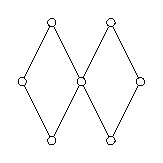
\includegraphics[width=.5\linewidth]{pictures/VCpocdelta1}
		\caption*{}
        \end{minipage}%
        \begin{minipage}{.5\textwidth}
                \centering
                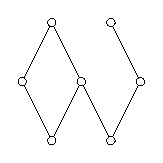
\includegraphics[width=.5\linewidth]{pictures/VCpocdelta2}
                \caption*{}
        \end{minipage}
        \caption{Graphs $\Delta_1$ and $\Delta_2$ from Theorem~\ref{pocVC:3}.}
	\label{pic:deltas}
\end{figure}
%%
%%
%%ToDo Only proof sketch of Theorem~\ref{pocVC:2}
%%
We will present two lemmata which are used in proofs of Theorem~\ref{pocVC:2} and Theorem~\ref{pocVC:3}.
These structural properties may be useful while trying to derive similar results for different values of the parameter \(t\).

\begin{lemma}[\citet{CambyCardinalFioriniSchaudt14}]
Let \(G\) be a connected graph and let \(C\) be a vertex cover of \(G\). 
Suppose	that \((\mathcal{A}, \mathcal{B})\) is a bipartition of the connected components of \(C\) with \(\mathcal{A}, \mathcal{B} \neq \emptyset\), then there
exist two components \(A\) and \(B\) each from different parts such that the number of vertices on the shortest path from \(A\) to \(B\) is 3.
\end{lemma}

\begin{myproof}
	Let us pick two components \(A \in \mathcal{A}\) and \(B \in \mathcal{B}\) with the minimum distance. 
	Such pair exists because \(C\) has a finite number of connected components.
	Path \(x_1, \dots, x_k\) is the shortest path between \(A\) and \(B\). Vertex \(x_1 \in A\) and \(x_k \in B\).
	On the contrary we suppose that \(k > 3\). 
	None of the vertices \(x_2, \dots x_{k-1}\) belong to \(C\). Otherwise, \(B\) is not the nearest component to \(A\).
	Edge \(x_2, x_3\) is not covered, but that contradicts that \(C\) is a vertex cover.
\end{myproof}

Let \(C\) be a vertex cover of a connected graph \(G\) and \(S\) be a connected component of \(C\).
Then \(P_C(S)\) denotes a set of vertices \(v \in V(G)\) such that \(N(v) \cap C \subseteq V(S)\).
In other words, \(P_C(S)\) contains \(S\) and vertices whose entire neighborhood is in \(S\).
In particular \(P_C(S)\) induces connected subgraph in \(G\).
\begin{lemma}[\citet{CambyCardinalFioriniSchaudt14}]
Let \(S_1, S_2, \dots, S_k\) be connected components of a
vertex cover \(C\). There exists at least one \(P_C(S_i)\) which is not a cutset of \(G\), i.e.
\(G[V(G) \setminus P_C(S_i)]\) is connected.
\end{lemma}

\begin{myproof}
	Sets \(P_C(S_i)\) are disjoint by definition.
	We define a new graph \(H\) with vertices corresponding to the sets \(P_C(S_i)\).
	Two vertices \(P_C(S_i)\) and \(P_C(S_j)\) are adjacent in \(H\) if neighborhoods of \(P_C(S_i)\) and \(P_C(S_j)\) 
	share at least one vertex.
	Formally:
	 \[V(H) = \{P_C(S_i): i \in \{1, \dots, k\}\}\]
	 and
	 \[E(H) = \{P_C(S_i), P_C(S_j)|  P_C(S_i) \cap P_C(S_j) \neq \emptyset\}.\]
	Since \(G\) is connected and \(C\) is a vertex cover, graph \(H\) is connected.
	Every connected graph contains at least one vertex that is not a cut vertex.
	Thus, in \(G\) there exists a set \(P_C(S_i)\) that is not a cutset. 
\end{myproof}

\section{PoC critical graphs for vertex cover}

\begin{defn}
A graph \(G\) is \emph{critical} if every induced subgraph \(H\) of \(G\) has strictly smaller price of connectivity than \(G\).
\end{defn}

Critical graphs are precisely those which can be listed in forbidden subgraphs characterization. Note that all previous examples of forbidden subgraphs are also critical.
In this section we will investigate structure of critical graphs in more detail.

Many proofs from this section will use the following inequality to derive a contradiction.

\begin{lemma}\label{VC:fracsum}
	Let \(\frac{a_1}{b_1}, \dots, \frac{a_i}{b_i}, \dots \frac{a_n}{b_n}\) be real fractions with positive denominator.
	Denote the largest and the smallest fraction \(M\) and \(m\) respectively.
	Then \[{m} \leq {\frac{\sum_{i=1}^{n}{a_i}}{\sum_{i=1}^{n}{b_i}}} \leq {M}\].
\end{lemma}

\begin{myproof}
	We observe that the following iquality holds:
	\[{a_1 + a_2 + \dots + a_n} = {b_1 q_1 + b_2 q_2 + \dots + b_n q_n},\] 
	where \(q_i\) is equal to \(\frac{a_i}{b_i}\).
	The expression on the right is clearly at most \((b_1 + \dots + b_n)M\) and at least \((b_1 + \dots + b_n)m\).
	To finish the proof it is enough to divide both sides of the inequality by the sum \(b_1 + \dots + b_n\).
\end{myproof}

\begin{lemma}[\citet{CambyCardinalFioriniSchaudt14}]\label{VC:Bridge}
Let \(G\) be a critical graph. An edge with both endpoints in the minimum size vertex cover cannot be a bridge in \(G\).
\end{lemma}
\begin{myproof}
	Suppose for the sake of contradiction that \(G\) has a minimum vertex cover with vertices \(x\), \(y\), such that edge \(xy\) is a bridge.
	This means that graph \(G \setminus (xy)\) has two connected components \(C_1\) and \(C_2\).
	\(C_1\) is adjacent only to \(x\) and \(C_2\) is adjacent only to \(y\).
	Consider two induced subgraphs \(H_1\) and \(H_2\) defined like this.
	The subgraph \(H_i\) contains \(C_i\) and vertices \(x\) and \(y\).
	The minimum vertex cover of \(G\) must have at least \(\tau(H_1) + \tau(H_2)\) vertices, because both vertices \(x\) and \(y\)  %%Vysvetlit lepe
	are in the minimum vertex cover of \(G\) and components \(C_1\) and \(C_2\) are disjoint.
	On the other hand, union of connected vertex covers of \(H_1\) and \(H_2\) is also a connected vertex cover of \(G\) because vertices \(x\), \(y\) are in the union
	and edge \(xy\) is a bridge.
	So number \(\tau_c(G)\) is at most \(\tau_c(H_1) + \tau_c(H_1)\).
	These inequalities together with Lemma~\ref{VC:fracsum} yields:
	\[{\frac{\tau(G)}{\tau_c(G)}} \leq {\frac{\tau(H_1) + \tau(H_2)}{\tau_c(H_1) + \tau_c(H_2)}} \leq {\max\left\{\frac{\tau(H_1)}{\tau_c(H_1)}, \frac{\tau(H_2)}{\tau_c(H_2)}\right\}}\]
	That contradicts the assumption that \(G\) is critical.
\end{myproof}

The technique demonstrated above allows us to derive further structural results about critical graphs.

\begin{lemma}\label{VC:IndNeig}
Let \(G\) be a critical graph, let a vertex \(x\) be an arbitrary vertex from a minimum size vertex cover. Then \(N(x)\) is an independent set.
\end{lemma}

%%Illustration of case on proof of Lemma~\ref{VC:IndNeig}
\begin{figure}
        \centering
        \begin{minipage}{.45\textwidth}
                \centering
                \def\offset{2}
\begin{tikzpicture}

                \tikzstyle{vertex}  = [circle, minimum width=4pt, draw, inner sep=0pt, fill=white]
                \node [vertex, label=above:{\scriptsize$x$},](x) at (2.5, 6) {};
                \node [vertex, label=below:{\scriptsize$u$}](u) at ({0 + \offset}, 3) {};
                \node [vertex, label=below:{\scriptsize$v$}](v) at ({1 + \offset}, 3) {};
                \draw ({0 + \offset + 0.5}, 2.2) ellipse (0.82cm and 1.4cm);
                \node (c) at ({0 + \offset + 0.5}, 0) {\scriptsize$C$};
                \draw (u) -- (v);
                \draw (u) -- (x);
                \draw (v) -- (x);
\end{tikzpicture}


                \caption*{First case}
        \end{minipage}%
        \begin{minipage}{.45\textwidth}
                \centering
                \def\offset{2}
\begin{tikzpicture}

                \tikzstyle{vertex}  = [circle, minimum width=4pt, draw, inner sep=0pt, fill=white]
                \node [vertex, label=above:{\scriptsize$x$},](x) at (3.5, 6) {};

                \foreach \i in {1,2}
                {
                        \ifnum \i = 2
                                \node [vertex, label=below:{\scriptsize$u_m$}](u\i) at ({2 + \i * \offset}, 3) {};
                                \node [vertex, label=below:{\scriptsize$v_m$}](v\i) at ({3 + \i * \offset}, 3) {};
                                \node [minimum size=2.5cm, minimum width = 7pt](dots) at ({((2 + \i * \offset) - ( 1 + (\i-1) * \offset))*0.5 + ((1 + (\i-1) * \offset))}, 3) {\huge{$\scriptstyle \cdots$}};

                                \draw ({2 + \i * \offset + 0.5}, 2.2) ellipse (0.82cm and 1.4cm);
                                \node (c\i) at ({2 + \i * \offset + 0.5}, 0) {\scriptsize$C_m$};



                        \else
                                \node [vertex, label=below:{\scriptsize$u_\i$}](u\i) at ({0 + \i * \offset}, 3) {};
                                \node [vertex, label=below:{\scriptsize$v_\i$}](v\i) at ({1 + \i * \offset}, 3) {};
                                \draw ({0 + \i * \offset + 0.5}, 2.2) ellipse (0.82cm and 1.4cm);
                                \node (c\i) at ({0 + \i * \offset + 0.5}, 0) {\scriptsize$C_\i$};


                        \fi

                        \draw (u\i) -- (v\i);
                        \draw (u\i) -- (x);
                        \draw (v\i) -- (x);


                }

\end{tikzpicture}


                \caption*{Second case}
        \end{minipage}
	\hfill
	\begin{minipage}{.45\textwidth}
                \centering
                \def\offset{2}
\begin{tikzpicture}
        \tikzstyle{vertex}  = [circle, minimum width=4pt, draw, inner sep=0pt, fill=white]
                \node [vertex, label=above:{\scriptsize$x$},](x) at (3.5, 6) {};

                \foreach \i in {1,2}
                {
                        \ifnum \i = 2
                                \node [vertex, label=below:{\scriptsize$u_m$}](u\i) at ({2.5 + \i * \offset}, 3) {};
                                \node [minimum size=2.5cm, minimum width = 7pt](dots) at
                                ({((2 + \i * \offset) - ( 1 + (\i-1) * \offset))*0.5 + ((1 + (\i-1) * \offset))}, 3) {\huge{$\scriptstyle \cdots$}};

                                \draw ({2 + \i * \offset + 0.5}, 2.2) ellipse (0.82cm and 1.4cm);
                                \node (c\i) at ({2 + \i * \offset + 0.5}, 0) {\scriptsize$C_m$};
                                \draw (u\i) -- (x);
                        \else
                                \node [vertex, label=below:{\scriptsize$u_\i$}](u\i) at ({0 + \i * \offset}, 3) {};
                                \node [vertex, label=below:{\scriptsize$v_\i$}](v\i) at ({1 + \i * \offset}, 3) {};
                                \draw ({0 + \i * \offset + 0.5}, 2.2) ellipse (0.82cm and 1.4cm);
                                \node (c\i) at ({0 + \i * \offset + 0.5}, 0) {\scriptsize$C_\i$};
                                \draw (u\i) -- (v\i);
                                \draw (u\i) -- (x);
                                \draw (v\i) -- (x);
                        \fi
                }
\end{tikzpicture}


                \caption*{Third case}
        \end{minipage}

	\caption{Illustration of the cases from the proof of Lemma~\ref{VC:IndNeig}.}
\end{figure}
\begin{proof}[Proof of Lemma \ref{VC:IndNeig}]
Let \(G\) be a critical graph and \(S\) a minimum vertex cover of \(G\) and vertex \(x \in S\).
For the sake of contradiction suppose there are two adjacent vertices \(u\) and \(v\) in \(G\) such that \(u, v \in N(x)\).
We will distinguish between these three cases.
\begin{enumerate}
\item The vertex \(x\) is not a cut vertex.
	
	Let \(H\) be the graph obtained by deleting of \(x\).
	Clearly \(\tau(G)\) is at most \(\tau(H) + 1\) because minimum vertex cover of \(H\) together with vertex \(x\) is a vertex cover of \(G\).
	The opposite inequality is also true. Notice that \(S \cap V(H)\) is a minimum vertex cover of \(H\). 
	A minimum connected vertex cover of \(H\) together with vertex \(x\) is also a connected vertex cover of \(G\).
	That is true because any vertex cover of \(H\) must include at least one vertex from the edge \(uv\) and both vertices are neighbors of \(x\). 
	Thus, \(\tau_c(G)\) can be bounded from above by this expression:
        	\[\tau_c(G) \leq {\tau_c(H}) + 1.\]
	Using these two inequalities and inequality from Lemma~\ref{VC:fracsum} gives us:	
		\[{\frac{\tau_c(G)}{\tau(G)}} \leq {\frac{\tau_c(H) + 1}{\tau(H) + 1}} \leq {\max\left\{ \frac{\tau_c(H)}{\tau(H)}, 1\right\}}.\]
	
	For every graph \(G\) the ratio between \(\tau\) and \(\tau_c\) is at least one.
	That means that the induced subgraph \(H\) of \(G\) satisfies \(\frac{\tau_c(G)}{\tau(G)} \leq {\frac {\tau_c(H)}{\tau(H)}}\).
	However, that contradicts the criticality of \(G\).
	
\item The vertex \(x\) is a cut vertex and each component in the graph \(G \setminus \{x\}\) has an edge in \(N(x)\).
	
	Denote these components \(C_1, C_2, \dots, C_m\).
	\begin{claim}
		\(\tau(G) = {\sum_{i = 1}^{m}{\tau(C_i)} + 1}\)
	\end{claim}
	The inequality \(\tau(G) \leq {\sum_{i = 1}^{m}{\tau(C_i)} + 1}\) is easy to see as the union of minimum vertex covers of \(C_i\) with vertex \(x\) is a vertex cover of the entire graph.
	
	Observe that \(S \cap V(C_i)\) is also a minimum vertex cover of \(C_i\). This implies the desired inequality.
		\[\tau(G) \geq {\sum_{i=1}^{m}{\tau(C_i)} + 1}.\]
	The claim is proved.
	
	We need to find an upper bound for a size of a minimum connected vertex cover of \(G\).
	The union of minimum connected vertex covers of \(C_i\) and vertex \(x\) make a connected vertex cover of \(G\).
	The reason is that each vertex cover of \(C_i\) contains at least one neighbor of \(x\) due to edges in \(V(C_i) \cap N(x)\).
	This yields the following upper bound:
		\[\tau_c(G) \leq {\sum_{i=1}^{m}{\tau_c(C_i)} + 1}.\]
	Let us combine all estimates together and then use Lemma~\ref{VC:fracsum}:

	\[\frac{\tau_c(G)}{\tau(G)} \leq {\frac{\tau_c(C_1) +, \dots, + \tau_c(C_m) + 1}{\tau(C_1) +,\dots, + \tau(C_m) + 1}} 
	\leq \max\left\{ \frac{\tau_c(C_i)}{\tau(C_i)}, 1\right\}.\]

	Again we have a contradiction with the assumption that \(G\) is critical.	

\item 
	The vertex \(x\) is a cut vertex and at least one component in \(G \setminus \{x\}\) does not have an edge in \(N(x)\).

	Additionally, we can assume that in \(G\) there is one component \(C_1\) with an edge \(uv\) in \(N(x)\). 
	The proof is complete otherwise.
	We denote such components \(C_1, \dots, C_m\).
	Consider all these induced subgraphs of \(G\): \(H_1\), \(C_1\), \dots, \(C_m\).
	Subgraph \(H_1\) includes all components without an edge in \(N(u)\) together with vertices \(x\) and \(u\).
	Without loss of generality we can assume that \(x\) is in some minimum vertex cover of \(H_1\). If it is not that the case that we know that in the minimum vertex cover is \(v\).
	We can switch \(v\) with vertex \(x\). Again this is a vertex cover of \(H_1\) because \(v\) is a leaf in \(H_1\).
	That implies that union of minimum vertex covers of \(H_1\) and \(C_i\) is a vertex cover of \(G\). 
	Conversely the size of minimum vertex cover of \(G\) is at least \(\tau(H_1) + \tau(C_1), + \dots, \tau(C_m)\).
	\(D \cap C_i\) is vertex cover of \(C_i\) and \(x\) is already counted in \(\tau(H_1)\).
	Observe that vertex \(x\) must be in any connected vertex cover of \(H_1\) because an edge \(xv\) needs to be covered and \(x\) is a cut vertex in \(H_1\).
	Also leaf \(v\) is not in any minimum connected vertex cover of \(H_1\). That means that in the sum of \(\tau_c\) of our subgraphs vertices \(x\) and \(v\)
	are counted no more than once.
	Using this and inequality from Lemma~\ref{VC:fracsum} we can estimate the ratio between \(\tau(G)\) and \(\tau_c(G)\) in the following way:	
	
	\[\frac{\tau_c(G)}{\tau(G)} \leq {\frac{\tau_c(H_1) + \tau_c(C_1) +, \dots, \tau(C_m)}{\tau(H_1) + \tau(C_1), + \dots, \tau(C_m) }} \leq 
	{\max\left\{ \frac{\tau_c(H_1)}{\tau(H_1)}, \frac{\tau_c(C_i)}{\tau(C_i)}\right\}}.\]

	This inequality implies that for one of the induced subgraphs \(H_1\) or \(C_i\) their price of connectivity is at least equal to \(\frac{\tau_c(G)}{\tau(G)}\), 
	but that contradicts assumption about criticality of \(G\). 
\end{enumerate}
\leavevmode
\end{proof}

\begin{lemma}\label{VC:1compNoEdge}
	Let \(G\) be a critical graph with \(\frac{\tau_c(G)}{\tau(G)} \geq \frac{3}{2}\) and 
	a minimum vertex cover contains two vertices \(x\), \(y\) such that \(G \setminus \{x, y\}\) is connected.
	Then \(N(x) \cup N(y)\) is an independent set. In particular \(xy \not\in E\).
\end{lemma}

\begin{myproof}
	Suppose that there is an edge between two vertices \(u \in N(x)\) and \(v \in N(y)\).
	Denote by \(G'\) graph obtained by deletion of vertices \(x\) and \(y\) from \(G\).
	Observe that \(\tau(G) \geq {\tau(G') + 2}\). 
	Any vertex cover of \(G\) without vertices \(x\) and \(y\) is a vertex cover of \(G'\) and vertices \(x\) and \(y\) belong to some minimum vertex cover of \(G\).
	From any connected vertex cover of \(G'\) it is possible to construct a connected vertex cover of \(G\) by adding vertices \(x\), \(y\), \(u\), \(v\).
	At least one of the vertices \(u\) and \(v\) is already in the connected minimum vertex cover so we can bound connected dominating number: \(\tau_c(G) \leq \tau_c(G') + 3\).
	\[\frac{\tau_c(G)}{\tau(G)} \leq {\frac{\tau_c(G') + 3}{\tau(G') + 2}}  \leq {\max\left\{ \frac{\tau_c(G')}{\tau(G')}, \frac{3}{2}\right\}}\]
\end{myproof}

If we know, that vertices \(x\) and \(y\) are adjacent, then condition for the ratio \(\frac{\tau_c(G)}{\tau(G)}\) can be omitted.

\begin{lemma}\label{VC:1compEdge}
        Let \(G\) be critical and minimum vertex cover contains two vertices \(x\), \(y\) such that \(G \setminus \{x, y\}\) is connected.
        Then \(N(x) \cup N(y)\) is an independent set.
\end{lemma}

\begin{myproof}
	Proof is nearly the same as for previous Lemma~\ref{VC:1compNoEdge}.
	The only difference is, that to transform a connected vertex cover of \(G'\) into a connected cover of the whole graph, it is enough to add only vertices \(x\), \(y\)
	and one vertex from the pair \(u, v\). 
	Since \(uv\) is an edge, at least one of the vertices \(u\) and \(v\) must be in any vertex cover of \(G'\).
	\[\frac{\tau_c(G)}{\tau(G)} \leq {\frac{\tau_c(G') + 2}{\tau(G') + 2}}  \leq {\max\left\{ \frac{\tau_c(G')}{\tau(G')}, 1\right\}}.\]
\end{myproof}

Now we turn our attention to the case, where graph \(G \setminus \{x, y\}\) has more than one component.
\begin{lemma}\label{VC:morecomp}
	Let \(G\) be critical with a minimum vertex cover \(S\).
	Suppose that \(S\) contains a pair of adjacent vertices \(x\), \(y\).
	Then set of vertices \(N(x) \cup N(y) \setminus \{x, y\}\) is an independent set.
\end{lemma}
To be able to prove this lemma we need to find out more about the structure of \(G\).
More precisely we want to reduce this problem to the case, where \(G \setminus {x, y}\) has only one component adjacent to both \(x\) and \(y\).

\begin{lemma}\label{VC:Char}
	Suppose that graph \(G\) is critical. Let \(S\) be a minimum vertex cover of \(G\) including vertices \(x\) and \(y\).
	Assume that there is at least one component \(C\) in \(G \setminus \{x, y\}\) such that a set of vertices \((N(x) \cup N(y)) \cap V(C)\) is independent.
	Then there is at most one component \(D\) with edges among vertices from \((N(x) \cup N(y)) \cap V(D)\), moreover vertices from \((N(x) \cup N(y)) \cap V(D)\)
	induce a complete bipartite subgraph in \(G\).
\end{lemma}

\begin{myproof}
	First let us show that \(G \setminus \{x, y\}\) contains at most one component \(D\) adjacent to both vertices \(x\) and \(y\)
	with edges in \(G[N(x) \cup N(y)]\).
	Suppose for the sake of contradiction that there are two such components, we will denote them \(D_1\) and \(D_2\).
	Pick one edge \(u_1v_1\) with both endpoints in \((N(x) \cup N(y)) \cap V(D_1)\) analogously pick an edge \(u_2, v_2\) in \((N(x) \cup N(y)) \cap V(D_2)\).
	Vertices \(u_1, u_2\) are from \(N(x)\) and \(v_1, v_2\) belong to \(N(y)\) (see Figure~\ref{pic:VCChar}). 
	A subgraph \(H\) is defined as: \[H:= G[V(G) \setminus V(D_1) \setminus V(D_2) \cup \{u_1, v_2\}]\]. 
	It consists of vertices \(u_1\), \(u_2\) and all remaining vertices outside the components \(D_i\).
	Consider induced subgraphs \(H\), \(D_1\) and \(D_2\). 
	\begin{claim}
		\(\tau(G) = \tau(H) + \tau(D_1) + \tau(D_2)\)
	\end{claim}
	We may choose minimum vertex covers of these subgraphs that are disjoint, moreover \(x\) and \(y\) are in a minimum vertex cover of \(H\). %%Tohle je divny
	Only problematic vertices are \(u_1\) and \(v_2\).
	Vertices \(u_1\) and \(v_2\) are leaves in \(H\), so they can be replaced by vertices \(x\) and \(y\).
	It is easy to see that the union of vertex covers of \(H\), \(D_1\) and \(D_2\) is a vertex cover of \(G\). 
	Thus, \[\tau(G) \leq \tau(H) + \tau(D_1) + \tau(D_2).\]
	The opposite inequality follows from the observation that sets \(S \cap V(D_1)\), \(S \cap V(D_2)\) and \(X \cap (H \setminus\{u_1, v_2\})\) 
	are vertex covers of \(D_1\), \(D_2\) and \(H\) respectively.
	
	\begin{claim}
		\(\tau_c(G) \leq \tau_c(H) + \tau_c(D_1) + \tau_c(D_2)\)
	\end{claim}
	The union of connected vertex covers of \(H\), \(D_1\) and \(D_2\) gives a connected vertex cover of \(G\). 
	Vertices \(x\) and \(y\) are in every connected vertex cover of \(H\) due to vertices \(u_1\), \(v_2\).
	Also any vertex cover of \(D_i\) must include a vertex from \(N(x) \cup N(y)\) because of edges \(u_iv_i\).
	So the inequality from the claim holds.
	
	Finally, we can use these estimates and the inequality from Lemma~\ref{VC:fracsum} to bound the price of connectivity of \(G\):
	
	\[\frac{\tau_c(G)}{\tau(G)} \leq {\frac{\tau_c(H) + \tau_c(D_1) + \tau_c(D_2)}{\tau(H) + \tau(D_1) + \tau(D_2)}} 
	\leq \max\left\{ \frac{\tau_c(H)}{\tau(H)}, \frac{\tau_c(D_i)}{\tau(D_i)}\right\}.\]
	At least one of the induced subgraphs \(H\), \(D_1\) and \(D_2\) has price of connectivity which is equal or greater than price of connectivity of \(G\)
	which contradicts the criticality of \(G\).

	It remains to prove, that vertices in \((N(x) \cup N(y)) \cap V(D)\) induce a complete bipartite graph.
	From Lemma~\ref{VC:IndNeig} we know that vertices from one neighborhood cannot 
	be adjacent to each other; thus, the graph has two parts: \(N(x)\) and \(N(y)\).
	Let us assume that there are there three vertices \(u, u' \in N(x)\) and vertex \(v \in N(y)\) s.t. \(u'v \not\in E\) and \(vu \in E\) (see Figure~\ref{pic:VCChar}).
	Induced subgraphs \(H\) includes vertices \(v\), \(u'\) and every vertex from \(V(G \setminus \{x, y\}) \setminus V(D)\).
	Similarly as before we consider induced subgraph \(H\) and \(D\).

	The rest of the proof follows the same strategy as before.
\end{myproof}

\begin{figure}
        \centering
        \begin{minipage}{.5\textwidth}
                \centering
                \def\xaxis{0.7}
\def\yaxis{1.5}
\def\offset{2}
        \begin{tikzpicture}

                \tikzstyle{vertex}  = [circle, minimum width=4pt, draw, inner sep=0pt, fill=white]
                \node [vertex, label=left:{\scriptsize$x$}](x) at (1, 3) {};
                \node [vertex, label=right:{\scriptsize$y$}](y) at (2, 3) {};
                \node (sc) at ($(x)!0.5!(y) + (0, -2)$) {\scriptsize$C$};
                \node [vertex, label=left:{\scriptsize$u_1$}](u1) at ($(x) + (-\offset, 2)$) {};
                \node [vertex, label=right:{\scriptsize$v_1$}](v1) at ($(y) + (-\offset, 2)$) {};
                \node [vertex, label=left:{\scriptsize$u_2$}](u2) at ($(x) + (\offset, 2)$) {};
                \node [vertex, label=right:{\scriptsize$v_2$}](v2) at ($(y) + (\offset, 2)$) {};

                %%Components C, D1, D2 
                \draw [fill=white](sc) ellipse (0.7cm and 1.2cm);
                \draw ($(u1)!0.5!(v1)$) ellipse (1.2cm and 0.7cm);
                \draw ($(u2)!0.5!(v2)$) ellipse (1.2cm and 0.7cm);

                %%Labels for components C and D1, D2
                \node (sc1) at ($(x)!0.5!(y) + (0, -2)$) {\scriptsize$C$};
                \node (d1) at ($(u1)!0.5!(v1) + (0, 0.25)$) {\scriptsize$D_1$};
                \node (d2) at ($(u2)!0.5!(v2) + (0, 0.25)$) {\scriptsize$D_2$};
                %%Edges
                \draw (x)--(y);
                \draw (u1)--(v1);
                \draw (u2)--(v2);
                \draw (x)--(u1);
                \draw (x)--(u2);
                \draw (y)--(v1);
                \draw (y)--(v2);
                \begin{scope}[on background layer]
                        \draw (x)--(sc);
                        \draw (y)--(sc);
                \end{scope}
        \end{tikzpicture}


                \caption*{}
        \end{minipage}%
        \begin{minipage}{.5\textwidth}
                \centering
                 \begin{tikzpicture}

                \tikzstyle{vertex}  = [circle, minimum width=4pt, draw, inner sep=0pt, fill=white]
                \node [vertex, label=left:{\scriptsize$x$}](x) at (1, 3) {};
                \node [vertex, label=right:{\scriptsize$y$}](y) at (2, 3) {};
                \node (sc) at ($(x)!0.5!(y) + (0, -2)$) {\scriptsize$C$};
                \node [vertex, label=above:{\scriptsize$v$}](v1) at ($(y) + (0, 2)$) {};
                \node [vertex, label=above:{\scriptsize$u'$}](u2) at ($(x) + (0, 2)$) {};
                \node [vertex, label=above:{\scriptsize$u$}](u1) at ($(u2)!0.5!(v1)$) {};


                %%Components C, D1, D2 
                \draw [fill=white](sc) ellipse (0.7cm and 1.2cm);
                \draw ($(u1) + (0, 0.4)$) ellipse (1.2cm and 0.7cm);

                %%Labels for components C and D1, D2
                \node (sc1) at ($(x)!0.5!(y) + (0, -2)$) {\scriptsize$C$};
                \node (d1) at ($(u1) + (0, 0.65)$) {\scriptsize$D$};
                %%Edges
                \draw (x)--(y);
                \draw (u1)--(v1);
                \draw (x)--(u1);
                \draw (x)--(u2);
                \draw (y)--(v1);
                \begin{scope}[on background layer]
                        \draw (x)--(sc);
                        \draw (y)--(sc);
                \end{scope}
\end{tikzpicture}


		\caption*{}
        \end{minipage}
	\caption{Graphs from proof of Lemma \ref{VC:Char}}
	\label{pic:VCChar}
\end{figure}

\begin{lemma}\label{VC:1comp}
	Let \(G\) be a critical graph with minimum vertex cover \(S\).
	Pick any two vertices \(x\) and \(y\) from \(S\).
	If \(G \setminus \{x, y\}\) contains one component \(D\) adjacent to \(x\) and \(y\) with an edge on \(N(x) \cup N(y)\),
	then there are no other components adjacent to both \(x\) and \(y\).
\end{lemma}

\begin{myproof}
	Suppose that there is a component \(C\) adjacent to \(x\) and \(y\).
	In \(D\) there exist an edge \(u, v\), where \(u \in N(x)\) and \(v \in N(y)\).
	Without loss of generality we can assume that vertex \(u\) is in \(S\).
	Consider graph \(G \setminus \{u, x\}\). 
	Vertices \(x\) and \(u\) have neighbors connected with an edge namely \(v\) and \(y\). 
	Vertex \(x\) has a neighbor \(w\) in the component \(C\) non-adjacent to \(u\).
	(See Figure~\ref{pic:1comp}.)
	
	Let us take two induced subgraphs \(H\) and \(D_1\) defined as follows.
	Subgraph \(D_1\) contains entire component \(C\), vertex \(y\), vertex \(v\) and connected component of \(D \setminus u\) containing \(v\).
	Especially vertices \(x\) and \(u\) are not included in \(D_1\). It is possible that \(D \setminus {u}\) is no longer connected. 
	Subgraph \(H\) is defined as: \(H := G[V(G) \setminus V(D_1) \cup \{u, w\}].\)
	In particular \(H\) contains \(x, y, u, w\).
	\begin{claim}
		The union of connected vertex covers of \(H\) and \(D_1\) is a connected vertex cover of \(G\).
	\end{claim}
	
	By choice of \(H\) vertices \(u\) and \(x\) are both in every minimum connected vertex cover of \(H\).
	Vertex \(y\) is a cut vertex in \(D_1\), it links components \(C\) and part of component \(D\) included in \(D_1\). 
	Thus, union of minimum connected vertex covers of \(H\) and \(D\) is connected vertex cover of \(G\) and the claim is proved.
	See figure~\ref{pic:1comp}

	
	To finish the proof we need to find an lower bound of \(\tau(G)\).
	Notice that \(S \cap D_1\) is vertex cover of \(D_1\) and \(S \cap H\) is vertex cover \(H\).
	Sets \(S \cap D_1\) and \(S \cap H\) are disjoint.
	Then this inequality follows: \(\tau(G) \geq {\tau(H) + \tau(D_1)}\).

	Using these facts and Lemma~\ref{VC:fracsum} it is possible to estimate the price of connectivity of \(G\) as:
	\[\frac{\tau_c(G)}{\tau(G)} \leq {\frac{\tau_c(H) + \tau_c(D}{\tau(H) + \tau(D)}} \leq {\max\left\{ \frac{\tau_c(H)}{\tau(H)}, \frac{\tau_c(D)}{\tau(D)}\right\}}.\]
	The last inequality yields contradiction with criticality of \(G\).
\end{myproof}

\begin{figure}
	\begin{minipage}{.45\textwidth}
                \centering
      		\def\width{1.65}
\def\height{-2.5}
\begin{tikzpicture}

                \tikzstyle{vertex}  = [circle, minimum width=4pt, draw, inner sep=0pt, fill=white]
                %%Components C and D
                \draw ({1.5}, 5.5) ellipse (2cm and 0.8cm);
                \draw [fill=white]({1.5}, 0.5) ellipse (2cm and 0.8cm);
		%%Vertices
		\node [vertex, label=left:{\scriptsize$x$}](x) at (1, 3) {};
                \node [vertex, label=right:{\scriptsize$y$}](y) at (2, 3) {};
                \node [vertex, label=left:{\scriptsize$u$}](u) at (1, 5) {};
                \node [vertex, label=right:{\scriptsize$v$}](v) at (2, 5) {};
                \node [vertex, label=left:{\scriptsize$w$}](w) at (1, 1) {};
                %%Labels for components C and D
                \node (d) at ({1.5}, 5.8) {\scriptsize$D$};
                \node (c) at ({1.5}, 0.8) {\scriptsize$C$};
		%%Edges
		\draw (x)--(y)--(v)--(u)--(x);
                \draw (x)--(w);

		\begin{scope}[on background layer]
                	\draw (y)--(2,1.2);
		\end{scope}
\end{tikzpicture}
 
		\caption*{}
        \end{minipage}
	\begin{minipage}{.45\textwidth}
                \centering
                \def\width{1.65}
\def\height{-2.5}
\begin{tikzpicture}
        \tikzstyle{vertex}  = [circle, minimum width=4pt, draw, inner sep=0pt, fill=white]
        \node [vertex, fill=black, label=left:{\scriptsize$u$}](u) at (1, 3) {};
        \node [vertex, fill=black, label=right:{\scriptsize$x$}](x) at (2, 3) {};
        \node [vertex, fill=black, label=above:{\scriptsize$y$}](y) at ($(x)!0.5!(u) + (0, 2)$) {};
        \node (z) at ($(y) + (-1.5, 0)$) {};
        \node [vertex, label=left:{\scriptsize$v$}](v) at ($(z) + (0, -0.5)$) {};
        \node [vertex, label=above:{\scriptsize$w$}](w) at ($(y) + (1.5, -0.5)$) {};
        \node (z2) at ($(y) + (1.5, 0)$) {};

        \draw[fill=white, rounded corners] ($(u) + (-\width, {\height})$) rectangle ($(x) + (\width, -0.65)$) {};
        \draw[rounded corners] ($(u) + (-\width, 1)$) rectangle ($(x) + (\width, -\height + 0.5)$) {};
        \draw ($(z)!0.5!(v)$) ellipse (0.6cm and 0.6cm);
        \draw ($(z2)!0.5!(w)$) ellipse (0.6cm and 0.6cm);
        %%Components labels
        \node (ld) at ($(z) + (0, 0.6)$) {\scriptsize$D'$};
        \node (lc) at ($(z2) + (0, 0.6)$) {\scriptsize$C$};
        \node (lD1) at ($(w) + (0, -0.8)$) {\scriptsize$D_1$};
	%%Edges
	\begin{scope}
		\draw (x)--(w);
        	\draw (u)--(x);
        	\draw (x)--(y);
        	\draw (u)--(v);
        	\draw (v)--(y);
		\draw (y)--(z2);
		\draw (x)--($(x) + (0.5, -0.65)$);
        	\draw (u)--($(u) + (-0.5, -0.65)$);
	\end{scope}
\end{tikzpicture}

                \caption*{}
        \end{minipage}
        \caption{Illustration of situation in proof of Lemma~\ref{VC:1comp}.}
	\label{pic:1comp}
\end{figure}
\begin{proof}[Proof of Lemma~\ref{VC:morecomp}]
	
	If the graph \(G \setminus \{x, y\}\) is connected then we are done with the proof according to Lemma~\ref{VC:1compEdge}.
	By Lemma~\ref{VC:Bridge}, Lemma~\ref{VC:Char} and Lemma~\ref{VC:1comp} the graph \(G\) has the following structure.
	In \(G\setminus \{x, y\}\) there is exactly one component \(D\) with an edge \(uv\), where \(u \in N(x)\) and \(v \in N(y)\)
	and all other components of \(G \setminus \{x, y\}\) are adjacent either to \(x\) or to \(y\). (See Figure~\ref{pic:morecomp}.) 
	In the same manner as before we focus on three induced subgraphs \(H_1\), \(H_2\) and \(D\) such that the vertices \(x,y\) 
	are in the union of connected vertex covers.
	Subgraph \(H_1\) contains components adjacent to \(x\), vertices \(x\) and \(u\)
	similarly, in \(H_2\) there are vertices \(y, v\) and components seeing only \(y\).
	Notice that sets \(S \cap V(H_1)\), \(S \cap V(H_2)\) and \(S \cap V(D)\) are vertex covers of \(H_1\), \(H_2\), \(D\), respectively.
	Thus, the vertex cover number of \(G\) is at least \(\tau(H_1) + \tau(H_2) + \tau(D)\).
		
	The union of connected vertex covers of the three subgraph is a connected vertex cover of \(G\).
	Vertex \(x\) is in every connected vertex cover of \(H_1\), \(y\) is in every connected vertex cover of \(H_2\) and at least one neighbor 
	of \(x\) or \(y\) is in the connected vertex cover of \(C\) due to edge \(uv\). This size of a minimum connected vertex cover of \(G\)
	is at most \(\tau_c(H_1) + \tau_c(H_2) + \tau_c(D)\).
	
	\[\frac{\tau_c(G)}{\tau(G)} \leq {\frac{\tau_c(H_1) + \tau_c(H_2) + \tau_c(D)}{\tau(H_1) + \tau(H_2) + \tau(D)}} 
	\leq {\max\left\{ \frac{\tau_c(H_1)}{\tau(H_1)}, \frac{\tau_c(H_2)}{\tau(H_2)}, \frac{\tau_c(D)}{\tau(D)}\right\}}.\]
	
	Using our estimates and Lemma~\ref{VC:fracsum} we derived inequality implying that one of the induced subgraphs has PoC at least equal to \(\frac{\tau_c(G)}{\tau(G)}\).
	However, that contradicts the assumption that \(G\) is critical.
\end{proof}

\begin{figure}
	\centering
	\def\width{1.65}
\def\height{-1.7}
\def\xdist{1}
\def\ydist{1}
\def\lbdist{0.23}
\begin{tikzpicture}
        \tikzstyle{vertex}  = [circle, minimum width=4pt, draw, inner sep=0pt, fill=white]
        \node [vertex, label=left:{\scriptsize$x$}](x) at (1, 1) {};
        \node [vertex, label=right:{\scriptsize$y$}](y) at (2, 1) {};
	\node [vertex, label=above:{\scriptsize$u$}](u) at ($(x) + (0, 3)$) {};
	\node [vertex, label=above:{\scriptsize$v$}](v) at ($(y) + (0, 3)$) {};
        %%Subgraphs
	\draw ($(u)!0.5!(v)$) ellipse (1.5cm and 0.6cm);
	\draw[rounded corners] ($(x) + (-\width, \height)$) rectangle ($(x) + (0.3, 1.5)$) {};
        \draw[rounded corners] ($(y) + (-0.3, \height)$) rectangle ($(y) + (\width, 1.5)$) {};
        %%Components
	\node (x1) at ($(x) + (-\xdist,  -\ydist)$) {};
	\node (x2) at ($(x) + (-\xdist,  \ydist)$) {};
	\node (ddx) at ($(x1)!0.5!(x2)$) {$\vdots$};
	\draw [fill=white](x1) ellipse (0.25cm and 0.35cm);
	\draw [fill=white](x2) ellipse (0.25cm and 0.35cm);
	
	\node (y1) at ($(y) + (\xdist,  -\ydist)$) {};
        \node (y2) at ($(y) + (\xdist,  \ydist)$) {};
        \node (ddy) at ($(y1)!0.5!(y2)$) {$\vdots$};
        \draw [fill=white](y1) ellipse (0.25cm and 0.35cm);
        \draw [fill=white](y2) ellipse (0.25cm and 0.35cm);

        %%Components labels
        \node (ld) at ($(v) + (0, 0.8)$) {\scriptsize$D$};
	%%\node (lh2) at ($(y) + (\width, 1.5) + (0,\lbdist)$) {\scriptsize$H_2$};
	%%\node (lh1) at ($(x) + (-\width + 0.3, 1.5 +\lbdist)$) {\scriptsize$H_1$};

        \begin{scope}[on background layer]
     		\draw (x)--(y);
        	\draw (u)--(v);
        	\draw (v)--(y); 
		\draw (u)--(x);
		\draw (x)--(x1);
		\draw (x)--(x2);
		\draw (y)--(y1);
		\draw (y)--(y2);
	\end{scope}
\end{tikzpicture}

        \caption{Illustration of situation in proof of Lemma~\ref{VC:morecomp}.}
        \label{pic:morecomp}
\end{figure}


\chapter{Price of connectivity for dominating set}\label{chap4}

\begin{defn}
A \emph{dominating set} of a graph \(G\) is a subset of vertices \(D\) such that every vertex has a neighbor in \(D\)
or is in \(D\).
The size of the smallest dominating set is denoted by \(\gamma_c(G)\) and a dominating set of this size is called \emph{minimum}.
\end{defn}

\begin{problem}
        \problemtitle{Dominating set (DS)}
        \probleminput{A graph \(G = (V,E)\) and a positive integer \(k\)}
        \problemquestion{Does \(G\) have a dominating set \(D\), such that \(|D| \leq  k\)?}
\end{problem}

The decision version of the dominating set problem for a given graph \(G\) is a well studied NP-problem. %%reference na tu ucebnici
To get acquainted with the problem, we show its NP-completeness by a reduction from vertex cover.

\begin{thm}
	The dominating set problem is NP-complete \cite{GareyJohnson79}.
\end{thm}
\begin{myproof}
We prove a slightly stronger statement: For every graph \(G\) there
exists a graph \(G'\) such that every vertex cover of \(G\) of size $k$ corresponds
to a vertex cover in \(G'\) of size \(k+1\), and that \(G'\) has a vertex cover of size at most $c$
if and only if \(G'\) has a dominating set of size at most $c$.

We first handle isolated vertices of \(G\), which always belong to a dominating set but never belong
to a vertex cover. Starting with \(G\), we construct a new graph \(G''\) that contains edges and vertices from \(G\) plus two additional vertices
\(x\) and \(y\). Additionally, we add the edge \(xy\) and an edge \(xv\) for every vertex \(v \in V(G)\).

Observe that \(G''\) has a vertex cover of size at most \(k + 1\) iff
\(G\) has a vertex cover of size at most \(k\), and that in \(G''\)
there are no more isolated vertices.

We construct our final graph \(G'\) as follows: To start, the graph \(G'\)
contains all vertices and edges from \(G''\).  For every edge \(uv\)
from \(E(G'')\), we add a new vertex \(w\) and edges \(uw\), \(vw\).  We
have to prove that \(G''\) has a vertex cover of size at most \(k\) if
and only if \(G'\) has a dominating set of size at most \(k\).  First,
suppose that \(G''\) has a vertex cover \(S\) of size \(k\).  The set
\(S\) contains at least one endpoint from each edge, so the original
vertices from \(G''\) are dominated.  The vertices representing edges of
the original graph are adjacent to two vertices, one of which is in
\(S\).  Thus, these vertices are also dominated.

Conversely, let \(D\) be a dominating set of \(G'\).  Notice that if
\(D\) includes a vertex \(w\) added for an edge \(uv\), we can replace
it by \(u\) or \(v\); we are allowed to do this as vertex \(w\)
dominates only \(u\), \(v\) and these three vertices induce a
triangle.  Since every additional vertex is dominated, such a modified
dominating set \(D\) contains at least one endpoint from every edge.
The set \(D'\) is vertex cover of size at most \(k\) of \(G''\).
\end{myproof}

\section{Dominating set and independence}
The size of a minimum dominating set that is also independent is called the \emph{independent domination number} and denoted by \(i(G)\).
The \emph{upper domination number} \(\Gamma(G)\) is the size of the largest minimal dominating set.
From these definitions we can immediately see that \(\gamma(G) \leq i(G) \leq \alpha(G)\).

\begin{obs}\label{DS:InDo}
	An independent set \(S\) is maximal independent if and only if it is independent and dominating.
\end{obs}
\begin{myproof}
	Suppose that \(S\) is a maximal independent set. For any vertex \(v\) from \(V(G) \setminus S\) the set \(S \cup \{v\}\) is no longer independent,
	which means that every vertex in \(V(G) \setminus S\) is adjacent to at least one vertex from \(S\).
	Hence, \(S\) is a dominating set.
	
	On the contrary, let \(S\) be a dominating and independent set and suppose that it is not maximal.
	There is a vertex \(u\) from \(V(G) \setminus S\) such that \(S \cup \{u\}\) is independent.
	However, \(S\) is not dominating because \(u\) does not share any edge with vertex from \(S\). 
	This is a contradiction.
\end{myproof}

Berge in his book \cite{Berge62} observed that a vertex set is maximal independent if it is minimal dominating set.

\begin{obs}[\cite{Berge62}]
	Every maximal independent set in a graph \(G\) is a minimal dominating set of \(G\).
\end{obs}

\begin{myproof}
	Let \(S\) be a maximal independent set in \(G\). By Observation~\ref{DS:InDo} \(S\) is a dominating set.
	For the sake of contradiction suppose that \(D\) is not a minimal dominating set.
	In \(S\) there is a vertex \(v\) such that the set \(S \setminus \{v\}\) is dominating.
	If the set \(S \setminus \{v\}\) dominates vertices from \(V \setminus S \setminus \{v\}\), then at least one vertex from
	\(S\) must be adjacent to \(v\) and \(S\) is not independent, which leads to a contradiction.
\end{myproof}

A direct corollary of this observation is the following inequality which is a part of the so-called \emph{domination chain}.
For more information on the chain we refer to Chapter 3 of the book \cite{HaynesHedetniemiSlater98} written by Haynes, Hedetniemi and Slayter.
\begin{cor}
	For any graph \(G\)\:
	\[\gamma(G) \leq i(G) \leq \alpha(G) \leq \Gamma(G).\]
\end{cor}

The domination chain does not need to be strict; if there is a graph \(G\) for which every induced subgraph \(H\) satisfies \(i(H) = \gamma(G)\),
we call such graph is called \emph{domination perfect}.
The domination perfect graphs were defined by Sumner and Moore in 1979~\cite{SummerMoore79} who were inspired by a notion of perfect graphs.
% Since then, there were several attempts to characterize this class.
The characterization of the class was open for some time. Finally, in 1995, Zverovich and Zverovich~\cite{ZverovichZverovich95} found a characterization in terms of 17 forbidden induced subgraphs.
Aside from the above, many other variants of domination are also investigated. The focus will be on one of them, namely connected domination.

\section{Connected dominating set}

\begin{defn}
	A \emph{connected dominating set} of a graph \(G\) is a dominating set \(D\) such that \(G[D]\) is connected.
	The size of the smallest dominating set is denoted by \(\gamma_c(G)\) and a connected dominating set of the size \(\tau_c(G)\) is called 
	a minimum connected dominating set.
\end{defn}

A connected dominating set can exist only in connected graphs (a DS must include at least one vertex from each connected component).
Sampathkumar and Walikar, who were among the first researchers investigating connected domination, observe in \cite{SampathkumarWalikar79}
the following property of the connected domination number:

\begin{thm}[\cite{SampathkumarWalikar79}]
	Let \(G\) be a graph and \(H\) its spanning subgraph.
	Then, \(\gamma_c(G) \leq \gamma_c(H)\).
\end{thm}

Another interesting property of connected dominating sets regarding spanning trees is the following.
\begin{thm}\cite{HedetniemiLaskar84}
	Let \(G\) be a graph on \(n \geq 3\) vertices.
	Denote the maximum number of leaves over all spanning trees of \(G\) by \(\epsilon_T(G)\).
	Then, \(\gamma_c(G) = {(n - \epsilon_T(G))} \leq n-2\).
\end{thm}

\begin{myproof}
	Let \(T\) be a spanning tree with \(\epsilon_T(G)\) vertices. Since \(T\) without leaves is a connected dominating set of \(G\)
	the following inequality follows: \(\gamma_c(G) \leq {n - \epsilon_T(G)}.\)
	
	Suppose that \(D\) is a connected dominating set of \(G\). 
	The set \(D\) is connected and thus it has a spanning tree \(T'\).
	We can add all vertices from \(V(G) \setminus D\) to \(T'\) in such a way that each remaining vertex has only one edge to \(T'\).
	We created a new spanning tree \(T\) of the entire graph \(G\). The number of added vertices is at most \(\epsilon_T(G)\).
	The size of a minimum connected dominating set is at least \({n - \epsilon_T(G)}\).
\end{myproof}

Camby and Schaudt discovered in \cite{CambySchaudt16} that any minimal connected dominating set in \(P_t\)-free graph
is either isomorphic to \(P_{t-2}\), or it does not contain \(P_{t-2}\) as an induced subgraph.
This theorem was used in several papers to design polynomial algorithms in \(P_t\)-free graphs.
Specifically, Johnson, Paesani and Paulusma~\cite{JohnsonPaesaniPaulusma20} use it to construct an efficient algorithm for finding a minimum connected vertex cover in \((sP_1 + P_5\))-free graphs
and Bonomo et. al.~\cite{Bonomo18} apply it to create a polynomial algorithm determining whether a given \(P_7\)-free graph is three colorable.
Moreover, in the same paper, Camby and Schaudt show that a connected dominating set with these properties can be found in polynomial time.

\begin{thm}\label{DS:P-2freeT}
	For all \(t \geq 3\), any connected \(P_t\)-free graph has a connected dominating set whose induced subgraph is either \(P_{t-2}\)-free, 
	or isomorphic to \(P_{t-2}\).
\end{thm}

We will not show their proof in its entirety. 
Instead we will explain to a reader a proof of a weaker lemma which is used in the original proof by Camby and Schaudt.
What is more, this lemma will come in handy later in proofs of Theorems~\ref{DSpoc:2} and \ref{DSpoc:3} characterizing Near-PoC-perfect graphs for dominating set.
\begin{lemma}\label{DS:P-2free}
Let \(G\) be a connected graph that is \((P_k , C_k )\)-free for some \(k \geq 4\) and
let \(X\) be a minimal connected dominating set of \(G\). Then \(G[X]\) is \(P_{k-2}\)-free.
\end{lemma}
\begin{myproof}
	Let \(X\) be a minimum connected dominating set of \(G\).
	On the contrary suppose that \(X\) contains an induce path \(v_1, \dots, v_{k-2}\).
	Look at the set \(X \setminus \{v_1\}\).
	Because \(X\) is a minimum dominating set, \(X \setminus \{v_1\}\) is not dominating or not connected.
	In the first case in \(G\) there is a vertex \(v'_1\) adjacent only to one vertex from \(X\):\(v_1\).
	
	In the second case vertices \(v_2, \dots, v_{k-2}\) are all in one connected component. 
	Vertex \(v_1\) has a neighbor \(v'_1\) in a different connected component.
	In both cases \(v_1\) has a neighbor that is not adjacent to any from the vertices \(v_2, \dots v_{k_2}\).
	We can use the same reasoning for a vertex \(v_{k-2}\).
	Vertices \(v'_1, v_1, \dots, v_{k-2}, v'_{k-2}\) induce path or cycle on \(k\) vertices which contradicts
	the fact that \(G\) is \((P_k, C_k)\)-free.
\end{myproof}

\section{Price of connectivity}
We can define price of connectivity for dominating set in the same way as we did for vertex cover in \Cref{chap3}.
\begin{defn}
	For a graph \(G\), the price of connectivity (PoC) for dominating set is defined as the ratio \(\frac{\gamma_c(G)}{\gamma(G)}\).
\end{defn}

\begin{obs}
	The price of connectivity for any graph lies in the interval \([1, 3)\).
\end{obs}

\begin{myproof}
	Let \(D\) be a dominating set of \(G\) such that \(G[D]\) consists of \(c\) connected components.
	To make \(D\) connected it is enough to add at most \(2c - 2\) vertices. The distance between vertices in \(D\) is at most \(2\),
	since \(D\) is dominating.
	Assume that minimum dominating set of \(D\) has size \(k\).
	Using the previous observation:
	\[\frac{\gamma_c(G)}{\gamma(G)} \leq {\frac{k(2c - 2)}{k}} \leq {\frac{c(2c-2)}{c}} = {\frac{3c - 2}{c}} < 3.\]
\end{myproof}
Paths and cycles are examples of graphs attaining these bounds. Analogously, we can define PoC-perfect and PoC-near-perfect graphs for the dominating set:

\begin{defn}
	Graph \(G\) is \emph{PoC-perfect} if for every subgraph \(H\) of \(G\) it holds \(\gamma_c(H) = \gamma(H)\).
\end{defn}

\begin{defn}
	Graph \(G\) is \emph{PoC-near-perfect} with a threshold \(t \in (1, 3)\) if for every subgraph \(H\) of \(G\) this inequality holds \(\frac{\gamma_c(H)}{\gamma(H)} \leq t\).
\end{defn}
Zverovich in \cite{Zverovich03} provides characterization of PoC-perfect graphs.
\begin{thm}[\citet{Zverovich03}]\label{DSpoc:1}
The following assertions are equivalent:
\begin{enumerate}
	\item For a given graph \(G\) and every connected subgraph \(H\) it holds: \(\gamma_c(H) = \gamma(H).\)
	\item Graph \(G\) is \((P_5, C_5)\)-free.
\end{enumerate}
\end{thm}
Camby and Schaudt continue this line of research and in \cite{CambySchaudt14} they give a forbidden subgraphs characterization of PoC-near-perfect graphs 
with \(\gamma_c(H) \leq {\gamma(H) + 1}\):
\begin{thm}[\citet{CambySchaudt14}]\label{DSpoc:2}
	For every connected subgraph \(H\) of a graph \(G\) the inequality \(\gamma_c(H) \leq {\gamma(H) + 1}\) holds if and only if
	\(G\) is \((P_6, C_6)\)-free.
\end{thm}

\begin{myproof}
It is easy to see that \(\gamma(C_6) = \gamma(P_6) = 2\) and \(\gamma_c(C_6) = \gamma_c(P_6) = 4\).
These two graphs violate the inequality \(\gamma_c(H) \leq {\gamma(H) + 1}\) and therefore they cannot be induced subgraphs of \(G\).

Assume that \(G\) is \((P_6, C_6)\)-free.
Consider any connected induced subgraph \(H\) of \(G\). Observe that \(H\) is also \((P_6, C_6)\)-free.
To prove the sufficiency of our condition, we need to show that \(H\) satisfies \(\gamma_c(H) \leq {\gamma(H) + 1}\).
Let \(D\) be a minimum dominating set of \(H\) with connected components \(D_1, \dots, D_k\).
The set \(D\) must have at least two connected components, otherwise \(\gamma_c(H) = \gamma(H)\) and we are done.
Consider the smallest set of vertices \(C\) such that \(H[D \cup C]\) is connected.
Denote \(X\) a minimum connected dominating set of \(H[D \cup C]\). We know that \(\gamma_c(H) \leq |X|\).
	Define the set of indices \(I = \{i \subseteq \{1, \dots, k\}: D_i \cap X = \emptyset\}\). For each \(i \in I\) consider \(x_i \in X\) such that
\(x_i\) is adjacent to a vertex from \(D_i\). Such vertex exists because \(X\) is dominating. The vertices \(x_i\) are all from \(C\)
and they do not have to be distinct.
Define the set \(S \subseteq X\):
	\[S = \bigcup_{i \not\in I}{D_i \cap X} \cup \{x_j: j \in I\}.\]
The size of \(S\) is by definition at most
	\[ \sum_{i \not\in I}{|D_i \cap X|} + |I|\]
and that is at most \(|D|\).
A minimum dominating set has to include at least one vertex from every component.

We distinguish between two cases according to connectivity of \(H[S]\).

Suppose that \(H[S]\) is connected. Then \(H[D \cup \{x_j : j \in I\}]\) is connected and \(C\) contains only vertices \(x_j\).
Recall that \(C\) is a minimal set with this property.
In this case \(X = S\) and this yields:
	\[\gamma_c(H) \leq |X| = |S| \leq {\sum_{i \not\in I}{|D_i \cap X|} + |I|} \leq |D| = \gamma(H).\]

\(H[S]\) is not connected.
By Lemma~\ref{DS:P-2free} \(H[X]\) is \(P_4\)-free. 
It is known that \(P_4\)-free graphs on at least two vertices are either disconnected or
their complement is disconnected \cite{Corneil81}
Specifically, it means that the graph \(\overline{H[S]}\) is connected.
Since \(H[X]\) is connected, the graph \(\overline{H[X]}\) is disconnected and it contains the set \(S\) in one connected component and a nonempty set of vertices \(Y\)
which are not adjacent to any vertex from \(S\).
What can we say about structure of graph \(H[X]\)? 
In \(X\), each vertex in \(Y\) is adjacent to every vertex from \(S\).
Thus, we can pick any vertex from \(y \in Y\) such that \(H[D \cup \{x_j: j \in I\} \cup \{y\}]\) is connected.
So \(|C| = \{x_j: j \in I\} \cup \{y\}\) and \(X = S \cup \{y\}\).
This gives us: 
	\[\gamma_c(H) \leq {|X| + 1} = {|S| + 1} \leq {\sum_{i \not\in I}{|D_i \cap X|} + |I| + 1} \leq {|D| + 1} = \gamma(H) + 1.\]
This concludes the proof.
\end{myproof}
To see that this bound is sharp, we consider the graphs \(F_k\) which are constructed from \(K_{1, k}\)
by subdividing every edge once. See Figure \ref{pic:fks} for an illustration.

\begin{figure}
        \centering
        \begin{minipage}{.5\textwidth}
                \centering
                \begin{tikzpicture}%%minDS

                \tikzstyle{vertex}  = [circle, minimum width=4pt, draw, inner sep=0pt, fill=white]
                \node [vertex](x) at (3,3) {};
                \foreach \i in {1,...,4}
                {
                        \node [vertex](a\i) at ($(x)+(({45 + \i*90}:2cm)$) {};
                        \node [vertex, fill=black](b\i) at ($(a\i)!0.5!(x)$) {};
                        \draw (b\i) -- (x);
                        \draw (a\i) -- (x);
                }
\end{tikzpicture}

                \caption*{}
        \end{minipage}%
        \begin{minipage}{.5\textwidth}
                \centering
                \begin{tikzpicture}%%minCDS
                \tikzstyle{vertex}  = [circle, minimum width=4pt, draw, inner sep=0pt, fill=white]
                \node [vertex, fill=black](x) at (3,3) {};
                \foreach \i in {1,...,4}
                {
                        \node [vertex](a\i) at ($(x)+(({45 + \i*90}:2cm)$) {};
                        \node [vertex, fill=black](b\i) at ($(a\i)!0.5!(x)$) {};
                        \draw (b\i) -- (x);
                        \draw (a\i) -- (x);
                }
\end{tikzpicture}

                \caption*{}
        \end{minipage}
	\caption{Graph \(F_k\) for \(k=4\)
	with minimum dominating set and minimum connected dominating set indicated by black vertices.}
        \label{pic:fks}
\end{figure}

Camby and Schaudt~\cite{CambySchaudt14} also attempt to characterize PoC-near-perfect graphs with a parameter \(t=2\),
presenting the following theorem:

\begin{thm}[\citet{CambySchaudt14}]\label{DSpoc3}
For every \((P_8 , C_8)\)-free graph \(G\), it holds that
	\(\gamma_c(G) \leq 2 \gamma(G).\)
\end{thm}
The same authors in \cite{CambySchaudt14} and in \cite{Camby19} proposed a conjecture how to characterize all PoC-near-perfect graphs
with parameter \(t = 2\). Recently Bonamy et al. in \cite{Bonamy18} prove that their conjecture was correct:
\begin{thm}[\citet{Bonamy18}]\label{DSpoc:3}
The following assertions are equivalent:
\begin{enumerate}
	\item For a graph \(G\) and every induced subgraph \(H\) it holds: \(\gamma_c(H) \leq 2\gamma(H).\)
	\item The graph \(G\) is \((C_9, P_9, F)\)-free.
\end{enumerate}
\end{thm}

\begin{figure}
	\centering
        %%\documentclass[tikz,border=3mm]{standalone}
%%\usetikzlibrary{shapes,snakes}
%%\usetikzlibrary{backgrounds}
%%\usetikzlibrary{calc}
%%\begin{document}
        \begin{tikzpicture}

               \begin{scope}[every node/.style={circle,thin,draw, fill=white}]
		\node (v) at (1, 1) {};
                \node (v1) at (0, 1) {};
                \node (v2) at (2, 2) {};
                \node (v3) at (2, 0) {};

                \foreach \y in {2,3}
		{
			\foreach \z in {1,2,3}{
				\node at ($(v\y)+(\z,0)$) {};
			}
		}
		\end{scope}

		\begin{scope}[on background layer][every node/.style={fill=white,circle}, every edge/.style={draw=red,very thick}]
			\draw (v2)-- ++(1,0)-- ++(1,0)-- ++(1,0);
                	\draw (v3)-- ++(1,0)-- ++(1,0)-- ++(1,0);
			\draw (v2)--(v3);
			\foreach \x in {1,...,3}
                        	\draw (v) -- (v\x);

		\end{scope}

	\end{tikzpicture}
%%\end{document}



	\caption{Graph \(F\) from Theorem~\ref{DSpoc:3}.}
	\label{DS:graphF}
\end{figure}
The remaining question is how to characterize PoC-near-perfect graphs for different values of parameter \(t\).
The construction of forbidden subgraphs from the previous theorems can be generalized in the following way:
\begin{defn}\label{DS:tk}
	Class of graphs \(\mathcal{T}_k\) consist of all graphs created as follows:
	\begin{itemize}
		\item Start with any tree on \(k\) vertices. Denote these nodes \(v_1, v_2, \dots, v_k\).
		\item Subdivide each edge twice.
		\item To each original leaf, we attach a new vertex (which becomes the new leaf).
		\item The vertices \(N(v_i)\) may be connected by new edges if \(v_i\) is not adjacent to a leaf. 
                  If at any point \(N(v_i)\) induces a connected graph, we add a new leaf to \(v_i\)
                  and we do not add any more edges into \(N(v_i)\).
		\item Finally, we may add a set $M$ of edges among leaves if $M$ is a (not necessarily maximal)
                  matching.
	\end{itemize}
\end{defn}

\begin{obs}\label{ds:7}
	For any graph \(G_k\) from \(\mathcal{T}_k\), the domination number \(\gamma\) is equal to \(k\)
	and \(\gamma_c(G_k) = 3k - 2\).
\end{obs}
\begin{myproof}
Observe that vertices \(v_i\) dominate all vertices from \(V(G_k)\), and so \(\gamma \leq k\).
Since the closed neighborhoods of individual vertices \(v_i\) are disjoint and any dominating set must
contain at least one vertex from each \(N[v_i]\), we have \(\gamma \geq k\).

The size of a minimum connected dominating set is at most \(3k-2\). 
Let us take a minimum dominating set that contains all vertices \(v_i\).
To make this dominating set connected, we need to add all vertices except leaves.
Number of edges in the initial tree is \(k - 1\), in the second step we added two vertices for each edge.
The total sum is \(k + (2k - 1) = 3k - 2\).

To finish the proof it remains to show that the size of a minimum connected dominating set is at least \(3k - 2\).
We consider a minimum connected dominating set \(D\).
If \(D\) contains all vertices \(v_i\) from the discussion above it follows that the size of \(D\) is at least \(3k-2\).

Assume that a vertex \(v_j\) is not in \(D\).
Moreover, we  suppose that \(v_j\) is adjacent to a leaf \(l_1\) and a vertex \(x_1\).
The situation is the following. 
The set \(D\) dominates \(l_1\); thus, there is a leaf \(l_2\) in \(D\) adjacent to \(l_1\).
From the construction of \(G_k\) we can see that all leaves are adjacent to the vertices \(v_i\).
In particular \(l_2\) is adjacent to a vertex \(v_m\). For an illustration see Figure~\ref{DS:DSTk}.
At least one vertex from a pair \(x_1\), \(l_1\) must be in \(D\), otherwise \(v_j\) is not dominated by \(D\).
Vertices \(l_2\), \(v_m\) and \(x_2\) are in \(D\).
Since edges on leaves induce a matching we can modify \(D\) in such a way that it includes \(v_j\)
and has at most the same size. Namely we \(D\) vertices \(v_j, x_1\) and remove \(l_1\).

Suppose that vertex \(v_j\) is not adjacent to any leaf.
In that case \(N(v_j)\) does not induce a connected subgraph.
Vertex \(v_j\) is dominated by a vertex \(w\). 
Denote by \(C_1\) a connected component of \(N(v_j)\).
In the neighborhood of \(v_j\) there is another connected component \(C_2\).
Denote by \(w'\) a vertex from \(D\) that has a neighbor in \(C_2\).
Such vertex exists because vertices from \(C_2\) needs to be dominated by \(D\).
Let \(w''\) be a common neighbor of vertices \(v_j\) and \(w'\).
Since subgraph \(H[D]\) is connected, it contains a path \(P\) from \(w\) to \(w'\).
The path \(P\) must contain an edge between two leaves \(l_1\) and \(l_2\).
We remove \(l_1\) and \(l_2\) from \(D\) and add vertices \(v_j\), \(w''\) instead.
Notice that such modified \(D\) is still a connected dominating set and
the size is at most the same as before.
For reference see Figure \ref{DS:DSTk}.
\end{myproof}

\begin{figure}
        \centering
	\begin{minipage}{.5\textwidth}
                \centering
                        \begin{tikzpicture}

		\tikzstyle{vertex}  = [circle, minimum width=4pt, draw, inner sep=0pt, fill=white]
		\node [vertex, label={left:$l_1$}](l1) at (0,0) {};
		\node [vertex, fill=red, label={right:$l_2$}](l2) at (1,0) {};
		\node [vertex, fill=red, label={right:$v_m$}](vm) at ($(l2) + (-45:1cm)$) {};
		\node [vertex, label={left:$v_j$}](vj) at ($(l1) + (135:1cm)$) {};
		\node [vertex, label={above:$x_1$}](x1) at ($(l2) + (95:1cm)$) {};
		\node [vertex, fill=red, label={above:$x_2$}](x2) at ($(x1) + (30:1cm)$) {};
		\draw (vm) -- (l2) -- (l1) -- (vj) -- (x1)--(x2);

	\end{tikzpicture}


		\caption*{}
        \end{minipage}%
	\begin{minipage}{.5\textwidth}
                \centering
                \begin{tikzpicture}

                \tikzstyle{vertex}  = [circle, minimum width=4pt, draw, inner sep=0pt, fill=white]
                \node [vertex, fill=red, label={left:$l_1$}](l1) at (0,0) {};
                \node [vertex, fill=red, label={right:$l_2$}](l2) at (1,0) {};
                \node [vertex, fill=red, label={left:$w$}](w) at ($(l1) + (110:1cm)$) {};
                \node [vertex, label={left:$v_j$}](vj) at ($(w) + (30:1cm)$) {};
                \node [vertex, label={above:$w^{''}$}](w1) at ($(vj) + (30:1cm)$) {};
                \node [vertex, fill=red, label={above:$w^{'}$}](w2) at ($(w1) + (30:1cm)$) {};
                \draw (l2) -- (l1);
		\draw  (w) -- (vj) -- (w1)--(w2);
		\draw [dashed] (w) -- (l1);
		\draw [dashed] (w2) -- (l2);
\end{tikzpicture}

                \caption*{}
        \end{minipage}%

	\caption{Illustration to the proof of Observation~\ref{ds:7}. Red vertices are in a connected dominating set \(D\)}
        \label{DS:DSTk}
\end{figure}

A direct corollary of this observation is that for any graph \(G_k\) from \(\mathcal{T}_k\) the ratio
\(\frac{\gamma_c(G)}{\gamma(G)}\) is at most \(3 - \frac{2}{k}\).
\begin{conj}[\citet{Bonamy18personal}]\label{DS:conj}
Let \(G\) be a graph.
For each subgraph \(H\) of \(G\) it holds: \({\frac{\gamma_c(H)}{\gamma(H)}} \leq {3 - \frac{2}{k - 1}}\)
if and only if \(G\) is \(\mathcal{T}_k\)-free.
\end{conj}
Let us look at graphs from \(\mathcal{T}_k\) for various values of \(k\).
\begin{itemize}
	\item \(k = 2.\)
		The class \(\mathcal{T}_2\) contains only graphs \(C_6\) and \(P_6\) which are forbidden subgraphs from Theorem~\ref{DSpoc:2}.
	\item \(k = 3.\)
		The class \(\mathcal{T}_3\) includes \(C_9\), \(P_9\), \(F\).
		Their PoC is \(\frac{7}{3}\) and they are forbidden subgraphs for graphs with PoC at most \(2\) from Theorem~\ref{DSpoc3}.
	\item \(k = 4.\)
		Some examples of graphs from  \(\mathcal{T}_4\) are \(P_{12}\), \(C_{12}\) and graphs derived from a star on \(4\) vertices (see Figure~\ref{pic:T4}).
\end{itemize}
\begin{figure}
        \centering
        \begin{minipage}{.5\textwidth}
                \centering
                \begin{tikzpicture}%%minDS

                \tikzstyle{vertex}  = [circle, minimum width=4pt, draw, inner sep=0pt, fill=white]
                \node [vertex, fill=black](v1) at (2,4) {};
                \node [vertex, fill=black](v2) at ($(v1)+(-30:3cm)$) {};
                \node [vertex, fill=black](v3) at ($(v1)+(-90:3cm)$) {};
                \node [vertex, fill=black](v4) at ($(v1)+(210:3cm)$) {};

                \foreach \i in {2,...,4}{
                        \node [vertex](x\i) at ($(v1)!0.33!(v\i)$) {};
                        \node [vertex](y\i) at ($(v1)!0.66!(v\i)$) {};
                        \node [vertex](l\i) at ($(v\i)+(0,-1)$){};
                        \draw (v1)--(x\i)--(y\i)--(v\i)--(l\i);
                }
\end{tikzpicture}


                \caption*{}
        \end{minipage}%
        \begin{minipage}{.5\textwidth}
                \centering
                \begin{tikzpicture}%%minCDS 
                \tikzstyle{vertex}  = [circle, minimum width=4pt, draw, inner sep=0pt, fill=white]
                \node [vertex, fill=black](v1) at (2,4) {};
                \node [vertex, fill=black](v2) at ($(v1)+(-30:3cm)$) {};
                \node [vertex, fill=black](v3) at ($(v1)+(-90:3cm)$) {};
                \node [vertex, fill=black](v4) at ($(v1)+(210:3cm)$) {};

                \foreach \i in {2,...,4}{
                        \node [vertex](x\i) at ($(v1)!0.33!(v\i)$) {};
                        \node [vertex](y\i) at ($(v1)!0.66!(v\i)$) {};
                        \node [vertex](l\i) at ($(v\i)+(0,-1)$){};
                        \draw (v1)--(x\i)--(y\i)--(v\i)--(l\i);
                }
                \draw (x2)--(x3);
                \draw (x3)--(x4);
                \node [vertex](l1) at ($(v1)+(30:1cm)$){};
                \draw (v1)--(l1);
\end{tikzpicture}


                \caption*{}
        \end{minipage}
        \caption{An example of graphs from \(\mathcal{T}_4\)
        with vertices \(v_i\) indicated by black vertices.}
        \label{pic:T4}
\end{figure}

Note that not all graphs from \(\mathcal{T}_i\) are necessary critical. 
The construction from \Cref{DS:tk} allows the existence of subgraphs with the PoC equal or greater than \(3 - \frac{3}{k}\), namely 
an addition of edges to the neighborhood of \(v_i\) together with edges between leaves can create long induced paths.
This fact does not contradict our conjecture, it only means that our characterization is not minimal.

Unfortunately we will show that \Cref{DS:conj} is not true even for \(k = 3\).
To establish that we will show construction of critical graphs with PoC greater than \(3 - \frac{3}{k-1}\) without forbidden subgraphs from \(\mathcal{T}_i\).
\begin{thm}\label{DSpoc:4}
Let \(G_d\) be a graph with \(\gamma(G_d) = d\) constructed like this:
\begin{itemize}
	\item Start with a star on \(k\) vertices with central vertex \(v\).
	\item Add edges such that \(N(v)\) induces \(K_{\ceil{\frac{d-1}{2}}, \floor{\frac{d-1}{2}}}\). 
	\item To every vertex from the bipartite graph add a path on three vertices.
\end{itemize}
	Then for \(d = 5\) and \(d > 6\), the graph \(G_d\) is critical and we have \(\frac{\gamma_c(G_d)}{\gamma(G_d)} = {3 - \frac{3}{d}}\).
\end{thm}

\begin{figure}
	 \centering
         %%\documentclass[tikz,border=3mm]{standalone}
%%\usetikzlibrary{shapes,snakes}
%%\usetikzlibrary{backgrounds}
%%\usetikzlibrary{calc}
%%\begin{document}
        \begin{tikzpicture}
                %%\tikzstyle{vertex}      = [circle, minimum width=4pt, draw, inner sep=0pt, fill=white]

               \begin{scope}[every node/.style={circle,thin,draw, fill=white}]
		\node (v) at (1, 1) {};
                \node (v1) at (0, 2) {};
                \node (v2) at (2, 2) {};
                \node (v3) at (2, 0) {};
		\node (v4) at (0, 0) {};

                \foreach \y in {2,3}
		{
			\foreach \z in {1,2,3}{
				\node at ($(v\y)+(\z,0)$) {};
			}
		}

		 \foreach \y in {1,4}
                {
                        \foreach \z in {1,2,3}{
                                \node at ($(v\y)-(\z,0)$) {};
                        }
                }

		\end{scope}

		\begin{scope}[on background layer][every node/.style={fill=white,circle}, every edge/.style={draw=red,very thick}]
			\draw (v2)-- ++(1,0)-- ++(1,0)-- ++(1,0);
                	\draw (v3)-- ++(1,0)-- ++(1,0)-- ++(1,0);
			\draw (v1)-- ++(-1,0)-- ++(-1,0)-- ++(-1,0);
			\draw (v4)-- ++(-1,0)-- ++(-1,0)-- ++(-1,0);

			\draw (v1)--(v2)--(v3)--(v4)--(v1);
			\foreach \x in {1,...,4}
                        	\draw (v) -- (v\x);

		\end{scope}

	\end{tikzpicture}
%\end{document}



	 \caption{An example of a graph from Theorem~\ref{DSpoc:4} for $d = 5$.}
\end{figure}

\begin{proof}
	The size of a minimum connected dominating set of graph \(G_d\) is \(3d - 3\). It must include two vertices from each \(P_3\) and the whole bipartite subgraph.
	The minimum dominating set contains one vertex from each \(P_3\) and vertex \(v\).
	
	It remains to prove that \(G_d\) is a critical graph.
	In other words, every proper subgraph \(H\) must have a strictly smaller PoC than \(G_d\). 
	Due to relatively simple structure of \(G_d\) we analyze all possibilities of the subgraphs.
	For the rest of the proof we assume that the subgraph \(H\) is connected; the price of connectivity
        is defined only for connected graphs.
	Before diving deeper into the case analysis, we wish introduce some notation.
	
	Vertices of graph \(G_d\) can be divided into the following sets:
	\begin{itemize}
		\item \(P:=\) the set of vertices from \(P_3\) added in the last step of the construction.
		\item \(B_1, B_2 :=\) the sets of vertices from each part of the bipartite graph from the second step.
		\item \(v :=\) the central vertex of \(G_k\).
	\end{itemize}
	The number of induced paths with at least two vertices in \(P \cap V(H)\) is denoted by \(l\),
	the number of paths with one vertex in \(P \cap V(H)\) is denoted by \(s\).

	We will distinguish between several cases according to the structure of the subgraph \(H\).
	\begin{enumerate}
		\item [Case 1.] \(H \cong P_9.\)

		The price of connectivity of \(P_9\) is equal to \(\frac{7}{3}\).
        	To ensure criticality of \(G_d\), we need to set the value \(d\) such that the PoC of \(P_9\) is smaller than the PoC of \(G_d\).
        	\[\frac{\gamma_c(G_d)}{\gamma(G_d)} > \frac{7}{3}.\] 
        	This inequality implies that \(d\) must be greater than \(4\).
		We observe that \(P_9\) is the longest possible induced path in \(G_d\).

		\item [Case 2.] \(V(H) \cap P = \emptyset.\)
			
		In this case \(\frac{\gamma_c(H)}{\gamma(H)} = 1\).
		Vertices from the bipartite subgraph are dominated by either the vertex \(v\), or at most two adjacent vertices.
	\end{enumerate}
		
		The set of vertices \(H \cap P\) is nonempty. What does a minimum dominating set of \(H\) look like?
		In any dominating set, there must be at least one vertex from \(P\) for each long path and at least one vertex from \(B\) to dominate the short path.
		The minimum connected dominating set contains at most two vertices from \(P\) and one vertex from \(B\) for each path in \(H \cap P\).
		We distinguish between the following cases according to the number of short paths and the presence of vertex \(v\) in \(H\).
	\begin{enumerate}
		\item[Case 3.] \(s = 0\) and \(v \in H\).
                Every long path and the vertex \(v\) needs to be dominated, and so the size of a minimum dominating set of \(H\) is at least \(l + 1\).
                Suppose that the vertices from a minimum CDS of \(H\) (which dominate the vertices on the long paths from \(P \cap H\))
                include some from both parts \(B_1\) and \(B_2\).
		Thus \(\gamma_c(H) \leq 3l\).

		\[\frac{\gamma_c(H)}{\gamma(H)} \leq {\frac{3l}{l + 1}} = {3 - \frac{3}{l + 1}}.\]\label{case3s=0a}

		The last expression is increasing in \(l\) and \(l \leq d + 1\), so it is at most \(3 - \frac{3}{d}\).
		For smaller values of \(l\) the PoC of \(H\) is strictly smaller than \(3 - \frac{3}{d}\).
		When \(l\) is equal to \(d - 1\), at least one long path has one vertex not in \(H\), otherwise \(H \cong G\).
		Thus, we can improve the bound to:
		\[\frac{3l - 1}{l + 1} \leq {3 - \frac{4}{d}} < {3 - \frac{3}{d}}.\]\label{case3s=0b}

		In case that vertices from \(B\) adjacent to vertices from \(P \cap H\) are from the same part \(B_i\),
		the CDS contains one additional vertex that connects vertices from \(B_i\).
		Thus,  \(\gamma_c(H) \leq 3l + 1\) and we have:
		
		\[\frac{\gamma_c(H)}{\gamma(H)} \leq {\frac{3l + 1}{l + 1}} = {3 - \frac{2}{l + 1}}.\]	
		The number of paths with vertices from \(V(H) \cap P\)\ is at most \(\ceil{\frac{d - 1}{2}}\), which we plug in:
		\[{3 - \frac{2}{l + 1}} \leq {3 - \frac{2}{\frac{d + 2}{2}}} = {3 - {\frac{4}{d + 2}}} < 3 - \frac{3}{d}.\]

		The rightmost inequality is satisfied for \(d > 6\).
		This bound is not sharp for odd \(d\).
		The number of long paths is at most \(\frac{d-1}{2}\). 
		Using this bound yields the same result as before for \(d > 3\).
	
		\item [Case 4.] \(s \geq 2\) and \(v \in H\).
		
		The size of the minimum dominating set is at least \(l + s\).
		In the same manner as before, we distinguish several cases according to the size of a minimum connected dominating set.
			\begin{itemize}
				\item \(\gamma_c(H) \leq {3l + s}\). We compute:

				\[\frac{\gamma_c(H)}{\gamma(H)} \leq {\frac{3l + s}{l + s}} = {3 - \frac{2s}{l + s}} \leq {3 - \frac{4}{d - 1}} < {3 - \frac{3}{d}}.\]
				We have used that \(s\) is at least two.
			
				\item \(\gamma_c(H) \leq {3l + s + 1}\). In this situation all paths are adjacent to vertices from the same part of \(B\):
				\[\frac{\gamma_c(H)}{\gamma(H)} \leq {\frac{3l + s + 1}{l + s}} = {3 - \frac{2s - 1}{l + s}} \leq {3 - \frac{3}{l + s}}.\]

				The number of paths is at most \(\frac{d}{2}\).
				\[{3 - \frac{3}{l + s}} \leq {3 - \frac{6}{d}} < {3 - \frac{3}{d}}.\]
			\end{itemize}

		\item  [Case 5.] \(s = 1\) and \(v \in H\). We distinguish three subcases:
		
			\begin{itemize}
			\item All long paths on vertices \(V(H) \cap P\) are adjacent to one part \(B_i\).
				
			For a minimum connected dominating set, the inequality \(\gamma_c(H) \leq 3l + 2\) holds.
			By assuming \(s = 1\), a minimum connected dominating set includes a vertex from \(B\) dominating the short path. 
			Aside from this vertex, a minimum CDS also contains at most 3 vertices from each long path and at most one vertex from \(B\). 
			In particular, if one extra vertex from \(B\) is needed, then all paths on vertices \(P \cap V(H)\) are adjacent to vertices either from \(B_1\), or \(B_2\).
                        We calculate:

			\[{\frac{\gamma_c(H)}{\gamma(H)}} \leq {\frac{3l + 1}{l + 1}} = {3 - \frac{4}{d}} \leq {3 - \frac{3}{d}}.\]
			The last inequality holds for \(d > 0\).
			
			\item \(P \cap H\) induce two \(P_3\) adjacent to different parts of \(B\), or all paths \(H[V(H) \cap P]\) are adjacent to \(B_i\).
		
			This assumption implies that the size of minimum dominating set is at least \(l + 2\).
			From our estimates it follows that
			\[{\frac{\gamma_c(H)}{\gamma(H)}} \leq {\frac{3l + 2}{l + 2}} = {3 - \frac{4}{d}} < {3 - \frac{3}{d}}.\]

			
			\item The paths of length 3 with vertices from \(P \cap H\) are adjacent to one part of \(B\).
			The size of a minimum connected dominating can be expressed by:
				\[\gamma_c(H) = {3l_3 + 2l_2 + 1},\]
				where \(l_3\) is the number of \(P_3\) and \(l_2\) the number of \(P_2\) in \(H[V(H) \cap P]\).
			By our assumption, \(l_3\) is at most \(\ceil{\frac{d - 1}{2}} \leq {\frac{d}{2}}\).
			Similarly \(l_2 \leq \frac{d-1}{2}\).
				\[\gamma_c(H) = {3\frac{d}{2} + 2\frac{d-1}{2} - 1} = {\frac{5}{2}d - 2}\].
			
			Vertex dominating short path cannot be counted twice. %%Ukazat graf s timhle odhadem
			Let us bound price of connectivity of \(H\)
				\[\frac{\frac{5}{2}d - 2}{l_3 + l_2 + 1} \leq {\frac{\frac {5}{2}d - 2}{d-1}} = 2 - \frac{d}{2(d-1)}.\]
			The rightmost expression is strictly less than \(3-\frac{3}{d}\) for \(d > 7\).
			For even \(d\) bound of \(\gamma_c(H)\) can be improved because \(l_3 \leq (d-1)/2\). %\frac{d-1}{2}.
			Using this bound instead yields the same result for \(d > 3\).
			\end{itemize}
	\end{enumerate}

        \goodbreak
	\begin{enumerate}
	\item [Case 6.]\(s = 0\) and \(v \not\in H\). We go through three subcases once more:
		\begin{itemize}
			\item The graph \(H[V(H) \cap P]\) contains at least one \(P_3\) and \(\gamma_c(H) \leq 3l\).
				Due to the \(P_3\) in \(H[V(H) \cap P]\), the size of a dominating set is at least \(l + 1\).
			\[\frac{\gamma_c(H)}{\gamma(H)} \leq {\frac{3l}{l + 1}} = 3 - \frac{3}{l + 1}\]
		
			For \(l < d - 1\), the rightmost expression is strictly less than price of connectivity  of \(H\).
			In the case when \(l = d\) and at least one long path is shorter than 3, we are done
			by Case 3.

			Assume that each path from \(H[V(H) \cap P]\) is \(P_3\) and \(l = d-1\).
			If this is the case then observe that size of minimum dominating set is equal to \(l + 2\).
				\[\frac{\gamma_c(H)}{\gamma(H)} \leq {\frac{3l}{l + 2}} = 3 - \frac{6}{d + 1} < 3-\frac{3}{d}\]
			The last inequality holds for all \(d\).	

			\item Paths from \(H[V(H) \cap P]\) are adjacent to vertices from one part of \(B\).
				
			\[\frac{\gamma_c(H)}{\gamma(H)} \leq {\frac{3l + 1}{l + 1}} = 3 - \frac{2}{l + 1} 
			\leq {3 - \frac{2}{\frac{d + 2}{2}}} = 3 - \frac{4}{d + 2} < 3 - \frac{3}{d}.\]

			Since all paths are adjacent to vertices from one part of \(B\) the number of long paths is at most 
			\(\frac{d}{2}\).
			The last inequality holds for \(d > 6\).
			For odd \(d\) the number \(l\) is at most \(\frac{d - 1}{2}\).
			Using this bound instead we derive the same result for \(d > 3\).

			\item All paths in \(H[V(H) \cap P]\) have length 2.

			\[\frac{\gamma_c(H)}{\gamma(H)} \leq {\frac{2l + 1}{l}} = 2 - \frac{1}{l}\]
			Inequality \(2 - \frac{1}{l} < 3 - \frac{3}{d}\) holds for \(d > 4\).
		\end{itemize}
	
	\item [Case 7.]\(s = 1\) and \(v \not\in H\).
		
		Follows the same proof from Case 5.

	\item [Case 8.] \(s \geq 2\) and \(v \not\in H\).
		
		This situation is identical to Case 4.
\end{enumerate}
\end{proof}
The price of connectivity of graphs from \(\mathcal{T}_4\) is \(\frac{5}{2}\).
We proved that \(G_5\) is critical; thus it cannot contain
induced subgraphs with PoC greater than \(\frac{12}{5}\). In particular it cannot contain graphs with PoC equal to \(\frac{5}{2}\).
The conjecture for \(k=4\) claims that PoC-near-perfect graphs for \(t=\frac{7}{3}\) are exactly \(\mathcal{T}_4\)-free graphs.
However, \(G_5\) is a graph with price of connectivity greater than \(\frac{7}{3}\).
Hence, we found an counterexample.

In general we can derive the following corollary.
\begin{cor}
	For \(k > 5\) graphs \(G_{k + 1}\) from \Cref{DSpoc:4} are \(\mathcal{T}_{k}\)-free.
\end{cor}
\begin{myproof}
	From \Cref{DSpoc:4} graphs \(G_{k + 1}\) are critical with price of connectivity equal to \(3 - \frac{3}{k+1}\).
	By \Cref{ds:7} the price of connectivity of graphs from \(\mathcal{T}_{k}\) is equal to \(3 - \frac{2}{k}\).
	The inequality \[{3 - \frac{3}{k+1}} < {3 - \frac{2}{k}}\]
	holds for \(k > 2\). 
	Thus, graphs from \(\mathcal{T}_{k}\) cannot be induced subgraphs of \(G_{k + 1}\).
\end{myproof}

\section{Conclusions}
\Cref{chap3} discussed the characterization of PoC-near-perfect graphs for vertex cover for \(t = 1, \frac{4}{3}, \frac{3}{2}\)
as given by Camby and Schaudt. The same authors propose a possible characterization of the PoC-near-perfect graphs for \(t \leq \frac{5}{3}\). 
One possible direction of future research may be try to prove their conjecture and find a list of forbidden subgraphs for different values of \(t\).
% We also investigate the structural properties of PoC-critical graphs. 
In the same chapter, we have discussed the structural properties of PoC-cricital graphs; namely we observe that vertices from any minimum vertex cover have an independent neighborhood.
We derive a similar result for a pair of adjacent vertices from a minimum vertex cover in \Cref{VC:morecomp}.
The remaining question is whether the same property holds even for non-adjacent pair of vertices \(x, y\).

In \Cref{chap4} we show critical graphs with the price of connectivity for a dominating set equal to \(3-\frac{3}{k}\).
From the results listed in \Cref{chap4} about PoC-near-perfect graphs that in the interval \((1, 3)\), there exist rational values of the price of connectivity that
cannot be attained by any PoC-near-perfect graph. 
Interesting research problem to examine further could be to specify for which values of the price of connectivity 
PoC-near-perfect graphs exist. 

Notice that all PoC-near-perfect graphs do not contain long paths. 
Their study may be helpful in a better understanding to the class of \(P_r\)-graphs.
Recall that one of the few general characterizations of \(P_r\)-graphs (Theorem~\ref{DS:P-2freeT})
was established during an investigation of PoC-near-perfect graphs.

%%\include{epilog}

%%% Bibliography
%%% Bibliography (literature used as a source)
%%%
%%% We employ bibTeX to construct the bibliography. It processes
%%% citations in the text (e.g., the \cite{...} macro) and looks up
%%% relevant entries in the bibliography.bib file.
%%%
%%% The \bibliographystyle command selects, which style will be used
%%% for references from the text. The argument in curly brackets is
%%% the name of the corresponding style file (*.bst). Both styles
%%% mentioned in this template are included in LaTeX distributions.

%%\bibliographystyle{plainnat}    %% Author (year)
\bibliographystyle{unsrtnat}     %% [number]

\renewcommand{\bibname}{Bibliography}

%%% Generate the bibliography. Beware that if you cited no works,
%%% the empty list will be omitted completely.

\bibliography{bibliography}

%%% If case you prefer to write the bibliography manually (without bibTeX),
%%% you can use the following. Please follow the ISO 690 standard and
%%% citation conventions of your field of research.

% \begin{thebibliography}{99}
%
% \bibitem{lamport94}
%   {\sc Lamport,} Leslie.
%   \emph{\LaTeX: A Document Preparation System}.
%   2nd edition.
%   Massachusetts: Addison Wesley, 1994.
%   ISBN 0-201-52983-1.
%
% \end{thebibliography}


%%% Figures used in the thesis (consider if this is needed)
%%\listoffigures

%%% Tables used in the thesis (consider if this is needed)
%%% In mathematical theses, it could be better to move the list of tables to the beginning of the thesis.
%%\listoftables

%%% Abbreviations used in the thesis, if any, including their explanation
%%% In mathematical theses, it could be better to move the list of abbreviations to the beginning of the thesis.
%%\chapwithtoc{List of Abbreviations}

%%% Attachments to the master thesis, if any. Each attachment must be
%%% referred to at least once from the text of the thesis. Attachments
%%% are numbered.
%%%
%%% The printed version should preferably contain attachments, which can be
%%% read (additional tables and charts, supplementary text, examples of
%%% program output, etc.). The electronic version is more suited for attachments
%%% which will likely be used in an electronic form rather than read (program
%%% source code, data files, interactive charts, etc.). Electronic attachments
%%% should be uploaded to SIS and optionally also included in the thesis on a~CD/DVD.
%%% Allowed file formats are specified in provision of the rector no. 72/2017.
%%\appendix
%%\chapter{Attachments}

%%\section{First Attachment}

\openright
\end{document}
